\documentclass[TS]{sesamanuel}

% modifications dans la classe (fichier sesamanuel.cls) :
% 	1) ligne 2873, la ligne de remise à zéro du compteur de chapitre a été commentée pour "themaG"
% 	2) création d'une boîte à connaître à la ligne 3471
%	3) ligne 2141 : définition de trois couleurs utilisé par les anciennes figures libreoffice
%	4) ligne 179 et 180 ajout de 2 lignes pour utiliser la police pazocal qui modifie les caractères calligraphiés en mode math
%		du coup : \mathcal{C} donne un C fortement calligraphié et \pazocal{C} donne l'habituel C calligraphié de mathcal
%	5) suppression du texte et du logo dans le titre des QCM d'autoévaluation "Ressources dispo sur sesamaths..." :
%		lignes 3117 et 4396 : commande \StringManuel est commentée
%		lignes 3122 et 4401 : je n'ai pas supprimé le \LogoManuel (une @) mais j'ai changé sa couleur de U4 à Blanc (à la ligne 2702)

% modifications dans le fichier commandesTikZ :
% lignes 31 et 32 pour ajouter la commande \circled qui entoure un caractère



%%%%%%%
%Rajouté le 12/06/2018 SV et BN pour compilation espace insécable sous linux 
\DeclareUnicodeCharacter{00A0}{~} %pour remplacer les espaces insécables
\DeclareUnicodeCharacter{2011}{-}
%\usepackage{pdfpages}
%%%%%%%

% a priori, après l'impression du livre, tout ce fichier devrait être
% fusionné avec la classe principale, dernière version

\AtBeginDocument{\color{Noir}}

\renewcommand*\StringPrerequis{Connaissances
  n\'ecessaires \`a ce chapitre}

\usepackage{textcomp,pgfplots}
% standalone ne gère pas graphicspath... hum...
\newcommand{\standalonepath}[1]{#1}
% Au début de chaque chapitre on redéfinira cette commande en
% indiquant le chemin

\frenchbsetup{og=«,fg=»,}

\renewcommand\PrefixeCorrection{Corrections/}
\DeclareRemLike{intuition}{Idée intuitive}
\DeclareRemLike{exemples}{Exemples}


\newcommand*\StringExemples{Exemples}
\makeatletter
\newcommand*\smc@cartoucheexemples{% au pluriel
  \begin{pspicture}(-\ExempleVRuleWidthFrame,0)
                 (\ExempleWidthFrame,\ExempleHeightFrame)
    \psframe*[linewidth=0pt,linecolor=ExempleEdgeFrameColor]
             (-\ExempleVRuleWidthFrame,-\ExempleHRuleWidthFrame)
             (\ExempleWidthFrame,\ExempleHeightFrame)
    \psframe*[linewidth=0pt,linecolor=ExempleBkgFrameColor]
             (0mm,-0mm)(\ExempleWidthFrame,\ExempleHeightFrame)
    \rput[B](\dimexpr\ExempleWidthFrame/2,0){%
      \ExempleTitleFont
      \textcolor{ExempleTitleColor}{\StringExemples}%
    }
  \end{pspicture}%
}

\newenvironment{exemples*1}[1][]{%
  \par\addvspace{\BeforeExempleVSpace}
  \let\correction\smc@one@exemplecorrection
  \let\itemize\smc@exempleitemize
  \let\enditemize\endsmc@exempleitemize
  \let\colitemize\smc@exemplecolitemize
  \let\endcolitemize\endsmc@exemplecolitemize
  \let\enumerate\smc@exempleenumerate
  \let\endenumerate\endsmc@exempleenumerate
  \let\colenumerate\smc@exemplecolenumerate
  \let\endcolenumerate\endsmc@exemplecolenumerate
  \let\partie\smc@nopartie
  \let\exercice\smc@noexercice
  \let\endexercice\endsmc@noexercice
  \let\corrige\smc@nocorrige
  \let\endcorrige\endsmc@nocorrige
  \def\smc@currpart{Exemple}%
  \hspace*{\dimexpr \SquareWidth*3}%
  \color{ExempleRuleColor}%
  \vrule width \RuleWidth
  \hspace*{\dimexpr \SquareWidth-\RuleWidth}%
  \minipage[t]{\dimexpr\linewidth-\SquareWidth*4-\ExtraMarginRight}
    \smc@cartoucheexemples
    \space
    \color{Noir}%
    \ignorespaces
}
{%
  \endminipage
  \par
}

\DeclareRemLike{consequence}{Conséquence}
\DeclareRemLike{rappel}{Rappel}
\DeclareRemLike{valeurspart}{Valeurs particulières}
%\DeclareRemLike{theoreme}{Théorème}
% \NewThema{SP}
%          {sp}
%          {stat. et probabilités}
%          {Stat. et probabilités}
%          {STATISTIQUES\\ PROBABILITÉS}
%          {PartieStatistique}
%          {PartieStatistique}

\NewThema{A}
         {a}
         {analyse}
         {Analyse}
         {ANALYSE}
         {PartieFonction}
         {A3}


% Attention, il faudra ajouter un renewcommand \ListeMethodesThemes
% pour afficher la liste des méthodes à la fin du livre

% Si ils veulent changer la couleur du numéro des exos des
% auto-évaluations il faudra aller voir
% \colorlet{CorrigeNumExerciceFrameBkg}{J1}
 
\newcommand{\N}{\mathbb{N}} 
\newcommand{\R}{\mathbb{R}}
\newcommand{\Z}{\mathbb{Z}}
\renewcommand{\cfrac}[2]{{\displaystyle\frac{%
  \vrule height10pt depth0pt width0pt #1}{#2}}%
  \kern-\nulldelimiterspace}
%\usepackage{casio-fx,ti83symbols}

\newcommand\renvoimethode[1]{%
  Méthode \ref{#1}, p.~\pageref{#1}%
}

\newcommand*\calculatrice{%
  \psframebox[framesep=1pt,linewidth=\LogoLineWidth,
              linecolor=TiceLineColor, fillstyle=solid,
              fillcolor=TiceBkgColor, framearc=0.6]{%
    \TiceFont
    \textcolor{TiceTextColor}{CALC}%
  }
}
\newcommand\calc{\calculatrice}

% Chapitre G1 et G3
\newcommand{\covec}[2]{\left(\begin{array}{c} #1\\#2\end{array}\right)}

% Chapitre G2
\usepackage{tipa}
\newcommand{\arc}[1]{%
  \setbox9=\hbox{#1}%
  \ooalign{\resizebox{\wd9}{\height}{\texttoptiebar{\phantom{A}}}\cr#1}}

% Chapitre A4


\DeclareMathOperator{\e}{e}
\renewcommand{\cosh}{\operatorname{ch}}
\renewcommand{\sinh}{\operatorname{sh}}
\renewcommand{\tanh}{\operatorname{th}}

\newcommand*{\StringLEMM}{LEMME\footnote{Un \MotDefinition{lemme}{} est un résultat préliminaire ou  intermédiaire qui intervient parfois dans la preuve d'un théorème lorsqu'elle est un peu longue.}}
\newcommand*{\StringLEMME}{LEMME}
\DeclareDefLike{lemme}{\StringLEMME}
\DeclareDefLike{lemm}{\StringLEMM}

\newcommand*{\StringPROPRIETA}{PROPRIÉTÉ (admise)}
\DeclareDefLike{proprieta}{\StringPROPRIETA}

\usepackage{wrapfig}

% Environnement général pour toutes les fiches
\newcommand\AnnexeTICE{%
  \ChangeAnnexe{C2}{A1}{G1}{Blanc}%
  \annexe{}%
}
% Déclaration de l'environnement pour une fiche
\DeclareTPLike{ficheTICE}{Fiche}
              {TPTopColor}
              {TPBottomColor}
              {TPTitleColor} 
% Définition d'une commande \souspartie pour les besoins de la fiche
% TICE. C'est la commande \partie un peu revue. Je crée les mêmes
% paramètres de contrôle que pour TPPartie en mettant TPSousPartie à
% la place.

\colorlet{TPSousPartieColor}{J1}
\colorlet{TPSousPartieBkgColor}{C2}
\colorlet{TPSousPartieNumColor}{Blanc}
\newcommand*\TPSousPartieFont{\fontsize{10}{12}\sffamily\bfseries}
\def\BeforeTPSousPartieVSpace{3mm plus1mm minus1mm}
\def\AfterTPSousPartieVSpace{0mm plus1mm}
\edef\TPSousPartieHSep{\the\dimexpr\ItemRuleWidth+1.5mm}

\newcommand*\souspartie[1]{%
  \colorlet{smc@curr@partiecolor}{TPSousPartieNumColor}%
  \colorlet{smc@curr@partiebkgcolor}{TPSousPartieBkgColor}%
  \let\smc@curr@partiefont\TPSousPartieFont
  \par\addvspace{\BeforeTPSousPartieVSpace}
  \leavevmode
  \psframe*[linecolor=smc@curr@partiebkgcolor]
           (0,\ItemRuleDepth)(\ItemRuleWidth,\ItemRuleHeight)
  \hspace*{\TPSousPartieHSep}%
  \textcolor{TPSousPartieColor}{\TPSousPartieFont #1}
  \par\nobreak\addvspace{\AfterTPSousPartieVSpace}
}%

\newcommand\RoseItalTice[1]{\emph{\textcolor{C2}{#1}}}

%%% La présentation d'un texte en vis à vis d'une image n'est pas tout
%%% à fait un habillage et la répétition de tels éléments risque de
%%% poser des problèmes. Il vaut mieux se faire son propre « habillage
%%% »
\newcommand\ImageDroite[2]{%
  % #1 = texte
  % #2 = image (ou autre)
  \setbox4=\hbox{#2}%
  \dimen4=\dimexpr\ht4+\dp4-0.7\baselineskip
  \par
  \begin{tabularx}{\linewidth}{@{}Xc@{}}
    #1 & \raisebox{-\dimen4}{#2} %\box4
  \end{tabularx}
  \par
}
\newcommand{\commandetice}[1]{%
  \bgroup
  \shorthandoff{;:!?}%
  \texttt{#1}%
  \egroup
}

\newcommand\touchecalc[1]{%
  \tikz[baseline=-0.5ex]{\node at (0,0) [rounded corners = 2pt, draw, line width=.25pt]
    {\footnotesize\textsf{#1}}}%
}

\DeclareFontFamily{U}{tipa}{}
\DeclareFontShape{U}{tipa}{m}{n}{<->tipa10}{}
\newcommand{\arc@char}{{\usefont{U}{tipa}{m}{n}\symbol{62}}}%

\newcommand{\overarc}[1]{\mathpalette\arc@arc{#1}}

\newcommand{\arc@arc}[2]{%
  \sbox0{$\m@th#1#2$}%
  \vbox{
    \hbox{\resizebox{\wd0}{\height}{\arc@char}}
    \nointerlineskip
    \box0
  }%
}

% Pour A2

\def\psThomae{\pst@object{psThomae}}
\def\psThomae@i(#1,#2){%
   \begin@ClosedObj
   \addto@pscode{
     \psk@dotsize
     1 1 500 {
       dup
       /ipSave ED
       /ip ED
       1 1 500 {
         dup
         /iqSave ED
         /iq ED
         {
           iq 0 le { exit } if
           ip iq mod
           /ip iq def
           /iq ED
         } loop
         ip 1 eq {
           \psk@dotsize
           \@nameuse{psds@\psk@dotstyle}
           \pst@usecolor\pslinecolor ipSave iqSave div 1 iqSave div 
\tx@ScreenCoor
           2 copy moveto Dot
         } if
       } for
     } for
   }%
   \end@ClosedObj%
}

\renewcommand\smc@AfficheListeMethodesTheme[2]{%
  \expandafter\ifx\csname ifsmc@lom#1\endcsname\iftrue
    \csname smc@thema#2Color\endcsname
    \expandafter\smc@bandeaulistemethodes
      \expandafter{\csname StringListeMethode#2\endcsname}
    \ifnum \smc@NombreColonnesListeMethodes=\@ne
      \@starttoc{lom#1}
    \else
      \begin{multicols}{\smc@NombreColonnesListeMethodes}
        \@starttoc{lom#1}
      \end{multicols}
    \fi
  \fi
  \newpage
}
\fancypagestyle{empty}{%
  \fancyhead{}
  \fancyfoot{}
} 

\renewcommand*\AfficheCorriges[1][\NombreColonnesCorriges]{%
  \clearpage
  \label{toutes-solutions}
  \pagestyle{corrige}
  \thispagestyle{firstcorrige}
  \rput[Bl](0,9mm){\CorrigeTitleFont \MakeUppercase{\StringCorriges}}
  \vspace*{-5mm}
  \begingroup
  \columnsep \dimexpr \SquareWidth*2
  \columnseprule \CorrigeRuleWidth
  \def\columnseprulecolor{\color{ExerciceColumnRuleColor}}%
  \xdef\smc@NbColonneCorrige{#1}%
  \begin{multicols*}{#1}
  \raggedcolumns
    \@starttoc{cor}%
  \end{multicols*}
  \endgroup
}


\renewcommand\smc@preinsertlexiquefinal[3][]{%
  \@ifmtarg{#1}%
    {\smc@sansdiacritique{#2}}%
    {\smc@sansdiacritique{#1}}%
  \ifcsname affiche-\smc@tri\endcsname
  \else
    \expandafter\gdef\csname affiche-\smc@tri\endcsname{true}%
    \@ifmtarg{#1}%
      {\smc@sansdiacritique{#2}}%
      {\smc@sansdiacritique{#1}}%
    \global\advance\smc@numlexique \@ne
    \@ifmtarg{#1}%
      {\smc@@preFirstUppercase#2\@nil#3\@nil}%
      {\expandafter\protected@xdef\csname
lexique\the\smc@numlexique\endcsname
        {%
          \protect\textcolor{LexiqueEntreeColor}{%
            \protect\LexiqueEntreeFont #2%
          }%
%%%       \space\hbox to4.4em{\rdotfill}\kern0em\penalty0
          ~%%%
          \hspace*{\LexiquePageWidth}\penalty0
          \hspace{-\LexiquePageWidth}\dotfill
          \ifnum\csname nb-\smc@tri\endcsname>\@ne
            \protect\emph{ Pages~\csname pages-\smc@tri\endcsname}%
          \else
            \protect\emph{ Page~\csname pages-\smc@tri\endcsname}%
          \fi
        }%
      }%
    \expandafter\xdef\csname tri\the\smc@numlexique\endcsname
      {\smc@tri}%
  \fi
}
\long\def\smc@@preFirstUppercase#1#2#3\@nil#4\@nil{%
  \def\smc@arg{#1}%
  \ifx\smc@arg\smc@IeC
    \expandafter\protected@xdef\csname lexique\the\smc@numlexique\endcsname
      {%
        \protect\textcolor{LexiqueEntreeColor}
        {%
          \protect\LexiqueEntreeFont
          \MakeUppercase{#1#2}%
          \MakeLowercase{#3}%
        }%
        %%% \space\hbox to4.4em{\rdotfill}\kern-0.44em\penalty0
        ~%%%
        \hspace*{\LexiquePageWidth}\penalty0
        \hspace{-\LexiquePageWidth}\rdotfill
        \ifnum\csname nb-\smc@tri\endcsname>\@ne
          \protect\emph{ Pages~\csname pages-\smc@tri\endcsname}%
        \else
          \protect\emph{ Page~\csname pages-\smc@tri\endcsname}%
        \fi
      }%
  \else
    \expandafter\protected@xdef\csname lexique\the\smc@numlexique\endcsname
      {%
        \protect\textcolor{LexiqueEntreeColor}
        {%
          \protect\LexiqueEntreeFont
          \MakeUppercase{#1}%
          \MakeLowercase{#2#3}%
        }%
%%%     \space\hbox to4.4em{\rdotfill}\kern-0.44em\penalty0
        ~%%%
        \hspace*{\LexiquePageWidth}\penalty0
        \hspace{-\LexiquePageWidth}\rdotfill
        \ifnum\csname nb-\smc@tri\endcsname>\@ne
          \protect\emph{ Pages~\csname pages-\smc@tri\endcsname}%
        \else
          \protect\emph{ Page~\csname pages-\smc@tri\endcsname}%
        \fi
      }%
  \fi
} 

\makeatother

%\input{G1/biton} % pour l'instant on garde sinon les corrigés ne sont
						% pas dans classés dans un dossier "correction"

\usepackage{esvect,cancel} 
\newcommand{\chapeaumelon}[1]{\stackrel{\Large \frown}{#1}}

%%%%%%%% pour les figures en tikz
\usepackage{tikz}
\usepackage{tkz-tab,tkz-euclide}
\usetkzobj{all}
\usepackage{pgf}
\usetikzlibrary{arrows}
\usetikzlibrary{patterns}  
\definecolor{CyanTikz40}{cmyk}{.4,0,0,0}
\definecolor{CyanTikz20}{cmyk}{.2,0,0,0}

\definecolor{B1prime}      {cmyk}{0.00, 1.00, 0.00, 0.50}
\definecolor{H1prime}      {cmyk}{0.50, 0.00, 1.00, 0.00}

\tikzstyle{general}         =[font=\fontsize{7.5}{9}\selectfont,line width=0.3mm, >=stealth, x=1cm, y=1cm,line cap=round, line join=round]
\tikzstyle{quadrillage}     =[line width=0.3mm, color=CyanTikz40]
\tikzstyle{quadrillageNIV2} =[line width=0.3mm, color=CyanTikz20]
\tikzstyle{quadrillage55}   =[line width=0.3mm, color=CyanTikz40, xstep=0.5, ystep=0.5]
\tikzstyle{cote}            =[line width=0.3mm, <->]
\tikzstyle{epais}           =[line width=0.5mm, line cap=butt]
\tikzstyle{tres epais}      =[line width=0.8mm, line cap=butt]
\tikzstyle{axe}             =[line width=0.3mm, ->, color=Noir, line cap=rect]
\newcommand{\quadrillageSeyes}[2]{%
  \draw[line width=0.3mm, color=A1!10, ystep=0.2, xstep=0.8] #1 grid #2;
  \draw[line width=0.3mm, color=A1!30, xstep=0.8, ystep=0.8] #1 grid #2;
}

% ajouter pour manuel Flo
\newcommand*\circled[1]{\tikz[baseline=(char.base)]{
	\node[shape=circle,draw,inner sep=1pt] (char) {#1};}}

\newcommand{\axeX}[4][0]{%
  \draw[axe] (#2,#1)--(#3,#1);
  \foreach \x in {#4} {\draw (\x,#1) node {\small $+$};
    \draw (\x,#1) node[below] {\small $\numprint{\x}$};
  }%
}
\newcommand{\axeY}[4][0]{%
  \draw[axe] (#1,#2)--(#1,#3);
  \foreach \y in {#4} {\draw (#1, \y) node {\small $+$};
    \draw (#1, \y) node[left] {\small $\numprint{\y}$};
  }%
}
\newcommand{\axeOI}[3][0]{%
  \draw[axe] (#2,#1)--(#3,#1);
  \draw (1,#1) node {\small $+$};
  \draw (1,#1) node[below] {\small $I$};
}
\newcommand{\axeOJ}[3][0]{%
  \draw[axe] (#1,#2)--(#1,#3);
  \draw (#1, 1) node {\small $+$};
  \draw (#1, 1) node[left] {\small $J$};
}
\newcommand{\axeXgraduation}[2][0]{%
  \foreach \x in {#2} {\draw (\x,#1) node {\small $+$};}%
}
\newcommand{\axeYgraduation}[2][0]{%
  \foreach \y in {#2} {\draw (#1, \y) node {\small $+$};}%
}
\newcommand{\origine}{%
  \draw (0,0) node[below left] {\small $0$};
}
\newcommand{\origineO}{%
  \draw (0,0) node[below left] {$O$};
}
\newcommand{\point}[4]{%
  \draw (#1,#2) node[#4] {$#3$};
}
\newcommand{\pointGraphique}[4]{%
  \draw (#1,#2) node[#4] {$#3$};
  \draw (#1,#2) node {$+$};
}
\newcommand{\pointFigure}[4]{
  \draw (#1,#2) node[#4] {$#3$};
  \draw (#1,#2) node {$\times$};
}
\newcommand{\pointC}[3]{
  \draw (#1) node[#3] {$#2$};
}
\newcommand{\pointCGraphique}[3]{
  \draw (#1) node[#3] {$#2$};
  \draw (#1) node {$+$};
}
\newcommand{\pointCFigure}[3]{
  \draw (#1) node[#3] {$#2$};
  \draw (#1) node {$\times$};
}



\graphicspath{%
  {ex1/figures/}%
  {LesVecteurs/figures/}%
  {GeometriePlane/figures/}%
  {Images/}%
}


% création d'un nouveau thème "calcul" pour le document
\NewThema{C}{c}{calcul}{Calcul}{}{PartieFonction}{A3}

\renewcommand\ListeMethodesThemes{{c}{C},{g}{G}}
\renewcommand*\StringListeMethode{M\'ethodes du livret 1}

% création d'un nouveau thème "Manuel" pour le sommaire
\NewThema{M}{m}{manuel}{Manuel}{MANUEL}{PartieFonction}{A3}

\begin{document}

%%%%%%%%%%%%%%%%%%%%%%
%Couverture inclusion page entière en eps
\pagestyle{empty}

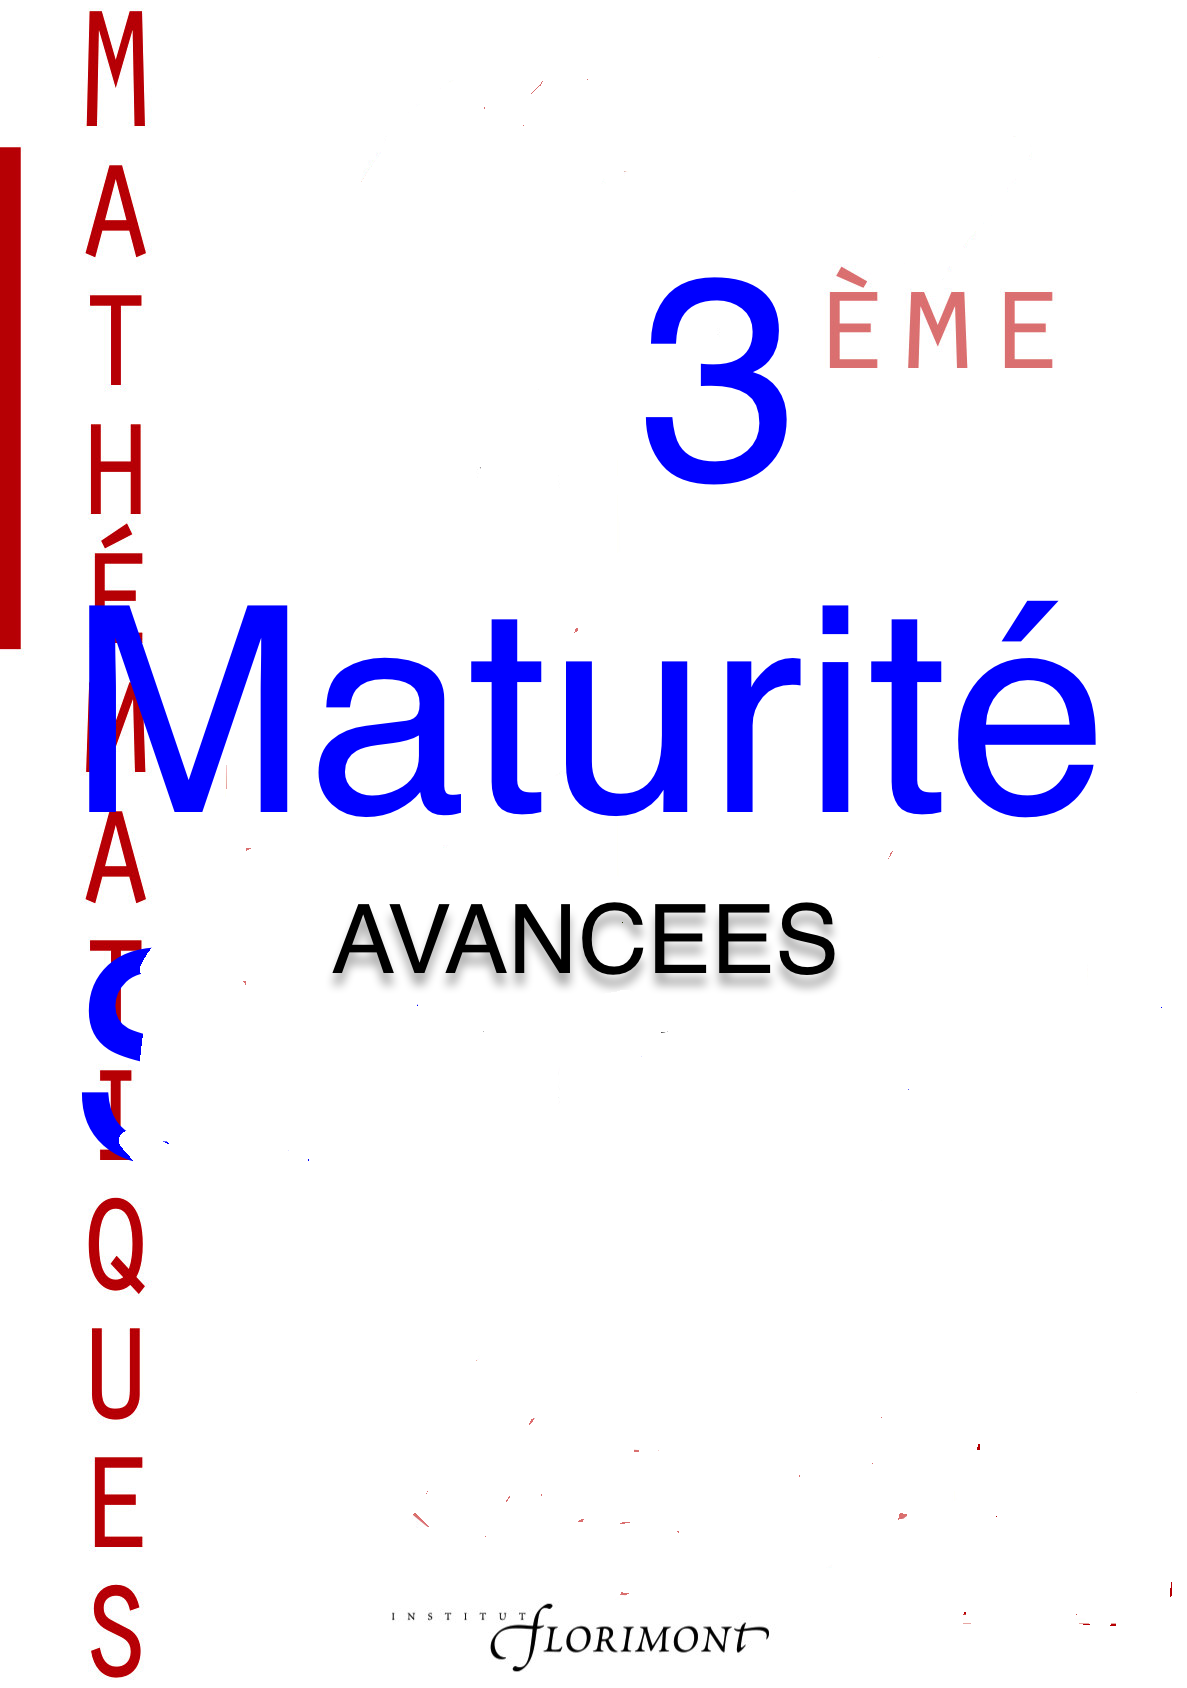
\includegraphics[width=.92\textwidth]{couverture}

\newpage \pagestyle{empty}
\addto\captionsfrench{\renewcommand{\contentsname}{Sommaire}}

%\setcounter{tocdepth}{2}


%%%%%%%%%%%%%%%%%%%%%%%%%%
% Table des matières
%%%%%%%%%%%%%%%%%%%%%%%%%%

\themaM %thème déclaré en début de document
\colorlet{ChapterNumColor}{PartieFonction}
\chapter{Manuel de\\Troisième Maturité\\Mathématiques Avancées}

\vfill

\begin{commentaire}

\textcolor{PartieFonction}{\PrerequisTitleFont 
Chapitre \ref{ChCalAlgebriques}: Calculs algébriques \dotfill\ page \pageref{ChCalAlgebriques}}

\vspace{2em}

\textcolor{PartieGeometrie}{\PrerequisTitleFont 
Chapitre \ref{ChLesVecteurs}: Les vecteurs 1 \dotfill\ page \pageref{ChLesVecteurs}}

\vspace{2em}

\textcolor{PartieFonction}{\PrerequisTitleFont 
Chapitre \ref{ChLesRacines}: Les racines nièmes \dotfill\ page \pageref{ChLesRacines}}

\vspace{2em}

\textcolor{PartieFonction}{\PrerequisTitleFont 
Chapitre \ref{ChEquations}: Les équations \dotfill\ page \pageref{ChLesEquations}}

\vspace{2em}

\textcolor{PartieGeometrie}{\PrerequisTitleFont 
Chapitre \ref{ChGeometriePlane}: Géométrie plane \dotfill\ page \pageref{ChGeometriePlane}

\vspace{2em}

\textcolor{PartieFonction}{\PrerequisTitleFont 
Chapitre \ref{ChInequations}: Inéquations \dotfill\ page \pageref{ChInequations}}

\vspace{2em}

\textcolor{PartieFonction}{\PrerequisTitleFont 
Chapitre \ref{ChPerimetresAires}: Nombres entiers et décimaux \dotfill\ page \pageref{ChPerimetresAires}}

\vspace{2em}

\end{commentaire}

\vfill

%%%%%%%%%%%%%%%%%%%%%%%%%%
% Fin table des matières
%%%%%%%%%%%%%%%%%%%%%%%%%%

%%%%%%%%%%%%%%%%%%%%%%%%%%
%Page Sesamath
%%%%%%%%%%%%%%%%%%%%%%%%%%
\newpage


\begin{prerequis}[Un manuel de l'association Sésamath]
\begin{itemize}
\item  Ce manuel est adapté en partie du manuel Sésamath de l'association Sésamath:\\
\texttt{http://manuel.sesamath.net/}
\item … Et de l'association Sésamath Suisse romande:\\ \texttt{http://www.sesamath.ch/}
\item L'Institut Florimont a réalisé la transcription dans le langage de description de documents libre et gratuit \LaTeX{} en utilisant la classe \texttt{sesamanuel} développée par l'association Sésamath;
\item E. Villié a réalisé la couverture pour l'Institut Florimont;
\item Version juin 2019 --- Institut Florimont (Genève).
\end{itemize}
 \end{prerequis}

\vspace{10em}




%%%%%%%%%%%%%%%%%%%%%%%%%%
%Fin page Sesamath
%%%%%%%%%%%%%%%%%%%%%%%%%%

\colorlet{ChapterNumColor}{white}
\setcounter{chapter}{0}

\themaC
\themaG


\setcounter{page}{6}

\themaC
\chapter{Calculs Algébriques}\label{ChCalculsAlgebriques}


\begin{acquis}
\begin{itemize}
\item Savoir calculer avec les puissances;
\item Savoir utiliser l'écriture scientifique;
\item Savoir développer une expression;
\item Savoir factoriser une expression en cherchant un facteur commun;
\item Savoir factoriser une expression en utilisant les identités remarquables.
\end{itemize}
\end{acquis}

\exercicesbase
\begin{colonne*exercice}
 \definecolor{fondTI}{HTML}{869286}


\serie{Développer et factoriser}

\begin{exercice}[]
Développer puis réduire les expressions suivantes :
\begin{enumerate}
\item $3a\times (4a-2ab+a^2c)$
\item $(2x-3xy)(4xy-5)$
\item $5-4(3-2x)(6-3x)-2[3-4x(5x+2)]-10(10x-9)$
\end{enumerate}
\end{exercice}
\medskip
\begin{exercice}[]
Factoriser puis simplifier les expressions suivantes :
\begin{enumerate}
\item $5a^2+10b-25ab$
\item $16x^4-24x^3+40x^2$
\item $2(2x-5)(4-3x)-(3+5x)(2x-5)+$

$4(2x+1)(2x-5)$
\item $5(4x-6)(5x+2)+3(7-2x)(10x-15)-2x+3$
\end{enumerate}
\end{exercice}
\medskip
\begin{exercice}[]
Factoriser les expressions suivantes en utilisant les identités remarquables :
\begin{multicols}{2}
\begin{enumerate}
\item $4y^2-24y+36$
\item $25+90x+81x^2$
\item $49y^2-81$
\item $x^2+12x+35$
\item $x^2+4x-32$
\item $-x^2+7x+8$
\item $x^2-10x+21$
\item $x^2-7x+6$
\item $-7x+30-x^2$
\end{enumerate}
\end{multicols}
\end{exercice}
\medskip
\begin{exercice}[]
Développer les expressions suivantes en utilisant les identités remarquables
\begin{enumerate}
\item $3+(8x+1)^2$
\item $12-(5+4x)^2$
\item $(8-9x)^2-6(24x+10)$
\item $(2x-1)(2x+1)-(x-4)(2x+5)$
\item $10+(x+5)(x+6)$
\item $(x-2)(x+4)-x(x+2)$
\item $(x-3)(x-6)+(x-3)^2$
\item $(3-2x)(3+2x)-9$
\end{enumerate}
\end{exercice}
\medskip
\begin{exercice}[]
Factoriser les expressions suivantes en utilisant les identités remarquables :
\begin{enumerate}
\item $(16x^2+24x+9)+2(4x+3)$
\item $(x+1)(7-2x)-(4x^2-28x+49)$
\item $4(6x-11)-(36x^2-121)$
\item $(3x-3)-(x^2-7x+6)$
\item $(x^2-3x-10)+(x^2-25)$
\item $x^4-1$
\end{enumerate}
\end{exercice}
\medskip
\begin{exercice}[]
Développer les expressions suivantes en utilisant le triangle de Pascal :
\begin{multicols}{2}
\begin{enumerate}
\item $(8x+1)^3$
\item $(3-2x)^4$
\item $(y+5)^5$
\item $(1-z)^6$
\item $(6-3t)^3$
\item $(7x+8)^4$
\end{enumerate}
\end{multicols}
\end{exercice}
\bigskip

\serie{Fractions algébriques}

\begin{exercice}[]
Simplifiez au maximum les fractions algébriques suivantes :

\begin{enumerate}
\item $\dfrac{2x^3-2xy^2}{4x^3-4x^2y}$
\item $\dfrac{x^2+5x+6}{x^2+4x+4}$
\item $\dfrac{x^2-y^2}{2x+2y}$
\item $\dfrac{x^2y+xy^2}{x^2+2xy+y^2}$
\item $\dfrac{2a^4-14a^3+20a^2}{a^4x-10a^3x+25a^2x}$
\end{enumerate}
\end{exercice}

\begin{exercice}[]
Calculer et simplifier au maximum les fractions algébriques suivantes :
\begin{enumerate}
\item $\dfrac{x^2-y^2}{z^-u^2} \times \dfrac{z-u}{x+y}$
\item $\dfrac{a^2-2ab}{x-y} \div \dfrac{a^2}{x^2-y^2} $
\item $\dfrac{x^2+10x+25}{x-3} \times \dfrac{5-x}{x^2-25}$
\item $\dfrac{a^2-b^2}{(2ab)^2} \div \dfrac{a+b}{2a}$
\end{enumerate}
\end{exercice}

\begin{exercice}[]
Calculer et simplifier au maximum les fractions algébriques suivantes :\\
\begin{enumerate}
\item $\dfrac{x}{x-4} + \dfrac{x-12}{2x-8}$
\item $\dfrac{x^3+x^2}{x^2+5x} - \dfrac{x^3-5x^2}{x^3-25x}$
\item $\dfrac{a+1}{2a-2} - \dfrac{a-1}{2a+2} - \dfrac{4a}{a^2-1}+ \dfrac{a^2+1}{a^2-1}$
\end{enumerate}
\end{exercice}




\end{colonne*exercice}

\connaissances
%

\QCMautoevaluation{Pour chaque question, plusieurs réponses sont % enlever le lien internet
  proposées.  Déterminer celles qui sont correctes.}

\begin{QCM}
  \begin{GroupeQCM}
    \begin{exercice}
      Le nombre $-4$ est \ldots
      \begin{ChoixQCM}{4}
      \item positif
      \item négatif
      \item l'opposé de $4$
      \item la valeur absolue de $4$
      \end{ChoixQCM}
\begin{corrige}
     \reponseQCM{bc} 
   \end{corrige}
    \end{exercice}
    
    
    \begin{exercice}
      Le nombre 3 est \ldots
      \begin{ChoixQCM}{4}
      \item positif
      \item négatif
      \item ni positif ni négatif
      \item l'opposé de $-3$
      \end{ChoixQCM}
\begin{corrige}
     \reponseQCM{ad} 
   \end{corrige}
    \end{exercice}


    \begin{exercice}
      La valeur absolue de $-10$ est \ldots
      \begin{ChoixQCM}{4}
      \item positive
      \item négative
      \item $-10$
      \item $10$
      \end{ChoixQCM}
\begin{corrige}
     \reponseQCM{ad} 
   \end{corrige}
    \end{exercice}


    \begin{exercice}
      L'abscisse de $A$ est \ldots 
\vspace{-2em}
\begin{center}  \includegraphics[width=2.6cm]{axeAB} \end{center}

      \begin{ChoixQCM}{4}
      \item $-1$
      \item $-2$
      \item positive
      \item négative
      \end{ChoixQCM}
\begin{corrige}
     \reponseQCM{ad} 
   \end{corrige}
    \end{exercice}
    
    
     \begin{exercice}
      Sur la droite précédente, l'abscisse de $B$ est \ldots
      \begin{ChoixQCM}{4}
      \item l'opposé de celle de $A$
      \item la valeur absolue de $-2$
      \item la valeur absolue de celle de $A$
      \item positive
      \end{ChoixQCM}
\begin{corrige}
     \reponseQCM{bd} 
   \end{corrige}
    \end{exercice}
    

    \begin{exercice}
      L'abscisse de $B$ est \ldots \hspace{0.4em} l'abscisse de $A$. 
      
\vspace{-2em}
\begin{center} \includegraphics[width=2.6cm]{axeBA} \end{center}

      \begin{ChoixQCM}{4}
      \item plus grande que
      \item plus petite que
      \item $>$
      \item $<$
      \end{ChoixQCM}
\begin{corrige}
     \reponseQCM{bd} 
   \end{corrige}
    \end{exercice}
    
 
     \begin{exercice}
      $-3$ est \ldots 3
      \begin{ChoixQCM}{4}
      \item plus grand que
      \item plus petit que
      \item la valeur absolue de
      \item l'opposé de
      \end{ChoixQCM}
\begin{corrige}
     \reponseQCM{bd} 
   \end{corrige}
    \end{exercice}
 \end{GroupeQCM}
\end{QCM}
 
 
\begin{QCM}
  \begin{GroupeQCM}   
    \begin{exercice}
      $-5$ \ldots $-7$
      \begin{ChoixQCM}{4}
      \item $>$
      \item $<$
      \end{ChoixQCM}
\begin{corrige}
     \reponseQCM{a}
   \end{corrige}
    \end{exercice}
    

    
    \begin{exercice}
      $-30$ \ldots $-35$
      \begin{ChoixQCM}{4}
      \item $>$
      \item $<$
      \end{ChoixQCM}
\begin{corrige}
     \reponseQCM{a}
   \end{corrige}
    \end{exercice}
    \begin{exercice}
      $-1,95$ \ldots $-1,94$
      \begin{ChoixQCM}{4}
      \item $>$
      \item $<$
      \end{ChoixQCM}
\begin{corrige}
     \reponseQCM{b}
   \end{corrige}
    \end{exercice}
    
    
    \begin{exercice}
      $-2,04$ \ldots $-2,048$
      \begin{ChoixQCM}{4}
      \item $>$
      \item $<$
      \end{ChoixQCM}
\begin{corrige}
     \reponseQCM{a}
   \end{corrige}
    \end{exercice} 

\end{GroupeQCM}
\end{QCM}

  


\pagebreak








\themaG
\chapter{Les vecteurs (1)}\label{ChLesVecteurs}

\begin{acquis}
\begin{itemize}
\item Connaitre la définition d'un vecteur, du vecteur nul;
\item Connaitre la définition de deux  vecteurs égaux, du milieu d'un segment;
\item Savoir utiliser la règle du parallélogramme, la relation de Chasles pour simplifier une expression comportant des vecteurs;
\item Savoir tracer la somme de deux vecteurs, le produit d'un vecteur par un réel;
\item Savoir montrer que deux vecteurs sont colinéaires.
\end{itemize}
\end{acquis}



\exercicesbase
\begin{colonne*exercice}

\serie{Egalité de vecteurs}

\begin{exercice}
Pour chaque paire de flèches, dire si elles sont le représentant d'un même vecteur ou pas. Justifier vos réponses en termes de : "direction", "sens" et "longueur".

\begin{center}
\definecolor{ffffff}{rgb}{1.,1.,1.}
\begin{tikzpicture}[scale=0.8][line cap=round,line join=round,>=triangle 45,x=1.0cm,y=1.0cm]
\clip(-4.3,-0.42) rectangle (5.76,6.3);
\draw [->] (-3.,5.) -- (-1.,5.);
\draw [->] (-2.,4.) -- (0.,4.);
\draw [->] (2.,5.) -- (4.,5.);
\draw [->] (5.,4.) -- (3.,4.);
\draw [->] (-3.,1.) -- (-2.,3.);
\draw [->] (-3.,1.) -- (-1.,0.);
\draw [->] (2.,2.) -- (5.,2.);
\draw [->] (3.,1.) -- (5.,1.);
\draw (-3.82,5.26) node[anchor=north west] {a)};
\draw (1.2,5.2) node[anchor=north west] {b)};
\draw (-3.76,2.24) node[anchor=north west] {c)};
\draw (1.2,2.22) node[anchor=north west] {d)};
\begin{scriptsize}
\draw [color=ffffff] (-3.,5.)-- ++(-0.5pt,-0.5pt) -- ++(1.0pt,1.0pt) ++(-1.0pt,0) -- ++(1.0pt,-1.0pt);
\draw [color=ffffff] (-1.,5.)-- ++(-0.5pt,-0.5pt) -- ++(1.0pt,1.0pt) ++(-1.0pt,0) -- ++(1.0pt,-1.0pt);
\draw [color=ffffff] (-2.,4.)-- ++(-0.5pt,-0.5pt) -- ++(1.0pt,1.0pt) ++(-1.0pt,0) -- ++(1.0pt,-1.0pt);
\draw [color=ffffff] (0.,4.)-- ++(-0.5pt,-0.5pt) -- ++(1.0pt,1.0pt) ++(-1.0pt,0) -- ++(1.0pt,-1.0pt);
\draw [color=ffffff] (2.,5.)-- ++(-0.5pt,-0.5pt) -- ++(1.0pt,1.0pt) ++(-1.0pt,0) -- ++(1.0pt,-1.0pt);
\draw [color=ffffff] (4.,5.)-- ++(-0.5pt,-0.5pt) -- ++(1.0pt,1.0pt) ++(-1.0pt,0) -- ++(1.0pt,-1.0pt);
\draw [color=ffffff] (5.,4.)-- ++(-0.5pt,-0.5pt) -- ++(1.0pt,1.0pt) ++(-1.0pt,0) -- ++(1.0pt,-1.0pt);
\draw [color=ffffff] (3.,4.)-- ++(-0.5pt,-0.5pt) -- ++(1.0pt,1.0pt) ++(-1.0pt,0) -- ++(1.0pt,-1.0pt);
\draw [color=ffffff] (-3.,1.)-- ++(-0.5pt,-0.5pt) -- ++(1.0pt,1.0pt) ++(-1.0pt,0) -- ++(1.0pt,-1.0pt);
\draw [color=ffffff] (-2.,3.)-- ++(-0.5pt,-0.5pt) -- ++(1.0pt,1.0pt) ++(-1.0pt,0) -- ++(1.0pt,-1.0pt);
\draw [color=ffffff] (-1.,0.)-- ++(-0.5pt,-0.5pt) -- ++(1.0pt,1.0pt) ++(-1.0pt,0) -- ++(1.0pt,-1.0pt);
\draw [color=ffffff] (2.,2.)-- ++(-0.5pt,-0.5pt) -- ++(1.0pt,1.0pt) ++(-1.0pt,0) -- ++(1.0pt,-1.0pt);
\draw [color=ffffff] (5.,2.)-- ++(-0.5pt,-0.5pt) -- ++(1.0pt,1.0pt) ++(-1.0pt,0) -- ++(1.0pt,-1.0pt);
\draw [color=ffffff] (3.,1.)-- ++(-0.5pt,-0.5pt) -- ++(1.0pt,1.0pt) ++(-1.0pt,0) -- ++(1.0pt,-1.0pt);
\draw [color=ffffff] (5.,1.)-- ++(-0.5pt,-0.5pt) -- ++(1.0pt,1.0pt) ++(-1.0pt,0) -- ++(1.0pt,-1.0pt);
\end{scriptsize}
\end{tikzpicture}
\end{center}

\end{exercice}

\begin{exercice}
Donner les caractéristiques des vecteurs suivants en fonction des caractéristiques du vecteur $\overrightarrow{v}$ : \\
\vspace{-5pt}
\begin{tabular}{p{3.5cm}p{3.5cm}}\\
\textbf{a)}$\overrightarrow{a}=\frac{1}{4}\overrightarrow{v}$&\textbf{b)}$\overrightarrow{c}=-\sqrt{5}\overrightarrow{v}$
\end{tabular}
\end{exercice}

\begin{exercice}

On considère les points  A, B, C, D, E et F

placés sur le quadrillage ci-dessous.

\vspace{0.25cm}
\begin{tikzpicture}[scale=0.65]
\draw [color=gray, xstep=1,ystep=1] (-0.5,-0.5) grid (8.5,6.5);
\begin{scriptsize}
\draw [color=black] (0.,0.)-- ++(-1.5pt,-1.5pt) -- ++(3.0pt,3.0pt) ++(-3.0pt,0) -- ++(3.0pt,-3.0pt);
\draw[color=black] (0.3,0.3) node {E};
\draw [color=black] (5.,0.)-- ++(-1.5pt,-1.5pt) -- ++(3.0pt,3.0pt) ++(-3.0pt,0) -- ++(3.0pt,-3.0pt);
\draw[color=black] (5.3,0.3) node {F};
\draw [color=black] (3.,3.)-- ++(-1.5pt,-1.5pt) -- ++(3.0pt,3.0pt) ++(-3.0pt,0) -- ++(3.0pt,-3.0pt);
\draw[color=black] (3.3,3.3) node {C};
\draw [color=black] (8.,3.)-- ++(-1.5pt,-1.5pt) -- ++(3.0pt,3.0pt) ++(-3.0pt,0) -- ++(3.0pt,-3.0pt);
\draw[color=black] (8.3,3.3) node {D};
\draw [color=black] (6.,6.)-- ++(-1.5pt,-1.5pt) -- ++(3.0pt,3.0pt) ++(-3.0pt,0) -- ++(3.0pt,-3.0pt);
\draw[color=black] (6.3,6.3) node {B};
\draw [color=black] (1.,6.)-- ++(-1.5pt,-1.5pt) -- ++(3.0pt,3.0pt) ++(-3.0pt,0) -- ++(3.0pt,-3.0pt);
\draw[color=black] (1.3,6.3) node {A};
\end{scriptsize}
\end{tikzpicture}


Dire si chacune des égalités suivantes est vraie

ou fausse.

\begin{multicols}{2}[\raggedcolumns]
\begin{enumerate}
\item $\overrightarrow{AB}=\overrightarrow{EF}$
\item $\overrightarrow{CD}=-\overrightarrow{AB}$
\item $\overrightarrow{DA}=\overrightarrow{DB}$
\item $\overrightarrow{ED}=\overrightarrow{BD}$
\item $\overrightarrow{AE}=\overrightarrow{BF}$
\item $\overrightarrow{EF}=-\overrightarrow{DC}$
\end{enumerate}
\end{multicols}
\end{exercice}

\begin{exercice}

\begin{enumerate}
\item Construire un triangle ABC tel que : AB = 3,5 cm, AC = 5 cm et BC = 4 cm.
\item Construire le point D tel que $\overrightarrow{CD}=\overrightarrow{AC}$   et le point E symétrique de B par rapport à C.
\item Quelle est la nature du quadrilatère ABDE ? Justifier votre réponse.
\end{enumerate}

\end{exercice}


\begin{exercice}

Soit ABCD et CDEF deux parallélogrammes.\\
Montrer que ABFE est aussi un parallélogramme.

\end{exercice}

\begin{exercice}
Soit [AB] un segment et I le milieu de [AB].\\
Déterminer dans chaque cas la valeur du réel $\alpha$ pour que l'égalité soit vraie :

\begin{multicols}{2}
\begin{enumerate}

\item $\overrightarrow{AI}=\alpha\overrightarrow{AB}$ ;
\item $\overrightarrow{AI}=\alpha\overrightarrow{IB}$ ;
\item $\overrightarrow{AB}=\alpha\overrightarrow{BI}$ ;
\item $\overrightarrow{AI}+\alpha\overrightarrow{IB}=\overrightarrow{0}$.

\end{enumerate}
\end{multicols}
\end{exercice}

\begin{exercice}
On considère un triangle quelconque $ABS$. On note $A'$ et $B'$ les symétriques respectifs de $A$ et $B$ par rapport à $S$.\\
Que peut-on dire des vecteurs $\overrightarrow{AB}$ et $\overrightarrow{A'B'}$? Justifier votre réponse.
\end{exercice}

\begin{exercice}
\begin{center}
\definecolor{cqcqcq}{rgb}{0.752941176471,0.752941176471,0.752941176471}
\begin{tikzpicture}[line cap=round,line join=round,>=triangle 45,x=1.0cm,y=1.0cm]
\draw [color=cqcqcq,dash pattern=on 2pt off 2pt, xstep=1.0cm,ystep=1.0cm] (-3.54,1.32) grid (3.7,5.66);
\clip(-3.54,1.32) rectangle (3.7,5.66);
\draw (-2.,5.)-- (3.,5.);
\draw (3.,5.)-- (2.,2.);
\draw (2.,2.)-- (-3.,2.);
\draw (-3.,2.)-- (-2.,5.);
\begin{scriptsize}
\draw [color=black] (-2.,5.)-- ++(-0.5pt,-0.5pt) -- ++(1.0pt,1.0pt) ++(-1.0pt,0) -- ++(1.0pt,-1.0pt);
\draw[color=black] (-2.,5.3) node {$A$};
\draw [color=black] (-3.,2.)-- ++(-0.5pt,-0.5pt) -- ++(1.0pt,1.0pt) ++(-1.0pt,0) -- ++(1.0pt,-1.0pt);
\draw[color=black] (-3.02,1.8) node {$B$};
\draw [color=black] (2.,2.)-- ++(-0.5pt,-0.5pt) -- ++(1.0pt,1.0pt) ++(-1.0pt,0) -- ++(1.0pt,-1.0pt);
\draw[color=black] (2.,1.84) node {$C$};
\draw [color=black] (3.,5.)-- ++(-0.5pt,-0.5pt) -- ++(1.0pt,1.0pt) ++(-1.0pt,0) -- ++(1.0pt,-1.0pt);
\draw[color=black] (3.02,5.32) node {$D$};
\end{scriptsize}
\end{tikzpicture}
\end{center}

\begin{enumerate}
\item Reproduire le parallélogramme ABCD ci-dessus puis construire les points E, F, G, H et I définis par :  $\overrightarrow{CE}=\overrightarrow{AC}$;  $\overrightarrow{BF}=\overrightarrow{AC}$;  $\overrightarrow{DG}=\overrightarrow{AC}$ ;  $\overrightarrow{AH}=-\overrightarrow{BC}$ ;  $\overrightarrow{IA}=\overrightarrow{AC}$
\item Quelle est la nature des quadrilatères BCEF et DGEC. Justifier votre réponse.
\item Que représente le point A pour le segment $[IC]$ ?Justifier votre réponse.
\end{enumerate}

\end{exercice}

\newpage

\serie{Opérations sur les vecteurs}

\begin{exercice}

\begin{center}
	\definecolor{qqqqff}{rgb}{0.,0.,1.}
\definecolor{cqcqcq}{rgb}{0.7529411764705882,0.7529411764705882,0.7529411764705882}
\begin{tikzpicture}[scale=0.6][line cap=round,line join=round,>=triangle 45,x=1.0cm,y=1.0cm]
\draw [color=cqcqcq,, xstep=1.0cm,ystep=1.0cm] (0.3,-3.5) grid (10.78,3.6);
\clip(0.3,-3.5) rectangle (10.78,3.6);
\draw [->] (1.,-3.) -- (3.,-1.);
\draw [->] (6.,-3.) -- (9.,-3.);
\draw [->] (8.,3.) -- (10.,0.);
\begin{scriptsize}
\draw [fill=qqqqff] (1.,-3.) circle (0.5pt);
\draw[color=qqqqff] (1.14,-2.64) node {$A$};
\draw [fill=qqqqff] (3.,-1.) circle (0.5pt);
\draw[color=qqqqff] (3.14,-0.64) node {$B$};
\draw[color=black] (2.,-1.7) node {$\overrightarrow{AB}$};
\draw [fill=qqqqff] (6.,-3.) circle (0.5pt);
\draw[color=qqqqff] (6.14,-2.64) node {$C$};
\draw [fill=qqqqff] (9.,-3.) circle (0.5pt);
\draw[color=qqqqff] (9.14,-2.64) node {$D$};
\draw[color=black] (7.56,-2.76) node {$\overrightarrow{CD}$};
\draw [fill=qqqqff] (8.,3.) circle (0.5pt);
\draw[color=qqqqff] (8.14,3.36) node {$E$};
\draw [fill=qqqqff] (10.,0.) circle (0.5pt);
\draw[color=qqqqff] (10.14,0.36) node {$F$};
\draw[color=black] (9.3,1.7) node {$\overrightarrow{EF}$};
\end{scriptsize}
\end{tikzpicture}
\end{center}

On considère les points $A$, $B$, $C$, $D$, $E$ et $F$ représentés ci-dessus. Reproduire les points et les vecteurs $\overrightarrow{AB}$, $\overrightarrow{CD}$ et $\overrightarrow{EF}$ sur votre cahier. Représenter de plus les vecteurs suivants :\\

\begin{tabular}{p{3.5cm}p{3.5cm}}
\textbf{a)} $\overrightarrow{a}=\overrightarrow{BC}$      & \textbf{e)} $\overrightarrow{e}=\overrightarrow{EF}+\overrightarrow{AB}$  \\\\
\textbf{b)} $\overrightarrow{b}=\overrightarrow{AB}+\overrightarrow{BC}$      & \textbf{f)} $\overrightarrow{f}=\overrightarrow{FE}+\overrightarrow{DC}$  \\\\
\textbf{c)} $\overrightarrow{c}=\overrightarrow{AB}+\overrightarrow{CD}$      & \textbf{g)} $\overrightarrow{g}=\overrightarrow{AB}+\overrightarrow{BC}+\overrightarrow{CD}$ \\\\
\textbf{d)} $\overrightarrow{d}=\overrightarrow{AB}+\overrightarrow{CB}$ 
\end{tabular}

\end{exercice}

\begin{exercice}
Construire un représentant des vecteurs suivants:
\begin{multicols}{2}
\begin{enumerate}
 \item $\overrightarrow{u}+\overrightarrow{AB}$
 \item $\overrightarrow{v}+\overrightarrow{CB}$
 \item $\overrightarrow{w} +\overrightarrow{DE}$
\end{enumerate}
\end{multicols}
   
\definecolor{qqqqff}{rgb}{0.,0.,1.}
\definecolor{cqcqcq}{rgb}{0.752941176471,0.752941176471,0.752941176471}
\begin{tikzpicture}[line cap=round,line join=round,>=triangle 45,x=1.0cm,y=1.0cm]
\draw [color=cqcqcq,dash pattern=on 2pt off 2pt, xstep=1.0cm,ystep=1.0cm] (-2.66,-2.64) grid (5.52,4.18);
\clip(-2.66,-2.64) rectangle (5.52,4.18);
\draw [->] (0.,2.) -- (2.,1.);
\draw [->] (5.,1.) -- (4.,-1.);
\draw [->] (-2.,0.) -- (-1.,1.);
\begin{scriptsize}
\draw [fill=qqqqff] (1.,-1.) circle (1.5pt);
\draw[color=qqqqff] (1.14,-0.72) node {$B$};
\draw [fill=qqqqff] (2.,1.) circle (1.5pt);
\draw[color=qqqqff] (2.14,1.28) node {$C$};
\draw [fill=qqqqff] (4.,2.) circle (1.5pt);
\draw[color=qqqqff] (4.14,2.28) node {$D$};
\draw [fill=qqqqff] (3.,-1.) circle (1.5pt);
\draw[color=qqqqff] (3.14,-0.72) node {$E$};
\draw[color=black] (1.08,1.74) node {$v$};
\draw[color=black] (4.74,0.14) node {$w$};
\draw [fill=qqqqff] (-2.,0.) circle (1.5pt);
\draw[color=qqqqff] (-2.2,0.26) node {$A$};
\draw[color=black] (-1.58,0.78) node {$u$};
\end{scriptsize}
\end{tikzpicture}
\end{exercice}

\begin{exercice}

En utilisant la relation de Chasles, simplifier au maximum les vecteurs suivants :
\begin{enumerate}

\item  $\overrightarrow{u}=\overrightarrow{AB}+\overrightarrow{BC}+\overrightarrow{CE}+\overrightarrow{EG}$
\item $\overrightarrow{w}=\overrightarrow{AB}+\overrightarrow{CB}+\overrightarrow{BD}+\overrightarrow{DE}$
\item  $\overrightarrow{v}=\overrightarrow{AB}+\overrightarrow{DA}+\overrightarrow{CD}+\overrightarrow{BC}$ 
\item $\overrightarrow{n}=\overrightarrow{AG}+\overrightarrow{DE}+\overrightarrow{CD}+\overrightarrow{GC}$

\end{enumerate}
\end{exercice}

\begin{exercice}

Sur chacune des figures suivantes, construire un représentant de $\vec{u}+\vec{v}$ :

\begin{enumerate}
\item \ \

\begin{tikzpicture}[scale=0.7]
\draw [-latex] (0.,0.) -- (4.,1.);
\draw [-latex] (0.,0.) -- (-2.,3.);
\begin{scriptsize}
\draw [color=black,thick] (0.,0.)-- ++(-2pt,-2pt) -- ++(4pt,4pt) ++(-4pt,0) -- ++(4pt,-4pt);
\draw (2,0.5) node[below] {$\vec{u}$};
\draw (-1,1.7) node[above] {$\vec{v}$};
\draw [color=white] (-3,5) circle (1pt);
\draw [color=white] (0,-2) circle (1pt);
\end{scriptsize}
\end{tikzpicture}

\item \ \

\begin{tikzpicture}[scale=0.75]
\draw [-latex] (0.,0.) -- (2.,4.);
\draw [-latex] (-2.,-1.) -- (3.,-2.);
\begin{scriptsize}
\draw [color=black,thick] (0.,0.)-- ++(-2pt,-2pt) -- ++(4pt,4pt) ++(-4pt,0) -- ++(4pt,-4pt);
\draw [color=black,thick] (-2,-1)-- ++(-2pt,-2pt) -- ++(4pt,4pt) ++(-4pt,0) -- ++(4pt,-4pt);
\draw (0.8,2) node[above] {$\vec{u}$};
\draw (0.5,-1.5) node[below] {$\vec{v}$};
\draw [color=white] (-3,3) circle (1pt);
\draw [color=white] (0,-4) circle (1pt);
\end{scriptsize}
\end{tikzpicture}

\end{enumerate}

\end{exercice}

\begin{exercice}
Sur chacune des figures suivantes, construire un représentant de $\vec{u}-\vec{v}$ :

\begin{enumerate}
\item \ \

\begin{tikzpicture}[scale=0.7]
\draw [-latex] (0.,0.) -- (4.,1.);
\draw [-latex] (0.,0.) -- (-2.,3.);
\begin{scriptsize}
\draw [color=black,thick] (0.,0.)-- ++(-2pt,-2pt) -- ++(4pt,4pt) ++(-4pt,0) -- ++(4pt,-4pt);
\draw (2,0.5) node[below] {$\vec{u}$};
\draw (-1,1.7) node[above] {$\vec{v}$};
\draw [color=white] (-3,5) circle (1pt);
\draw [color=white] (0,-2) circle (1pt);
\end{scriptsize}
\end{tikzpicture}

\item \ \

\begin{tikzpicture}[scale=0.75]
\draw [-latex] (0.,0.) -- (2.,4.);
\draw [-latex] (-2.,-1.) -- (3.,-2.);
\begin{scriptsize}
\draw [color=black,thick] (0.,0.)-- ++(-2pt,-2pt) -- ++(4pt,4pt) ++(-4pt,0) -- ++(4pt,-4pt);
\draw [color=black,thick] (-2,-1)-- ++(-2pt,-2pt) -- ++(4pt,4pt) ++(-4pt,0) -- ++(4pt,-4pt);
\draw (0.8,2) node[above] {$\vec{u}$};
\draw (0.5,-1.5) node[below] {$\vec{v}$};
\draw [color=white] (-3,3) circle (1pt);
\draw [color=white] (0,-4) circle (1pt);
\end{scriptsize}
\end{tikzpicture}

\end{enumerate}
\end{exercice}

\begin{exercice}
En utilisant la relation de Chasles, simplifier au maximum les vecteurs suivants :
\begin{enumerate}
\item $\overrightarrow{w}=-\overrightarrow{ED}-\overrightarrow{CB}+\overrightarrow{CD}-\overrightarrow{BA}$\\

\item $\overrightarrow{t}=\overrightarrow{BA}-\overrightarrow{CB}-\overrightarrow{ED}-\overrightarrow{DC}-\overrightarrow{FE}$\\

\item $\overrightarrow{s}=2\overrightarrow{AB}+3\overrightarrow{BC}+\overrightarrow{CD}$\\

 \item $\overrightarrow{n}=-\overrightarrow{BC}-\overrightarrow{DC}+\overrightarrow{DE}+2\overrightarrow{EB}$    \\
 
 \item $\overrightarrow{p}=2\overrightarrow{CD}+10\overrightarrow{DC}+10\overrightarrow{CE}-8\overrightarrow{DE}$ 
 \end{enumerate}
\end{exercice}

\begin{exercice}
Soient $A$, $B$, $C$, $D$ et $E$ des points du plan. En utilisant la relation de Chasles, simplifiez le plus possible les expressions suivantes : 
\begin{enumerate}

\item $\overrightarrow{BC}+\overrightarrow{CD}+\overrightarrow{DE}+\overrightarrow{EF}$    \\\\
\item $\overrightarrow{AB}+\overrightarrow{BC}+\overrightarrow{CD}$ \\\\    
\item $\overrightarrow{EA}-\overrightarrow{EB}-\overrightarrow{CE}-\overrightarrow{BC}$\\\\
\item $2\overrightarrow{AB}-2\overrightarrow{CB}$\\\\
\item $\overrightarrow{AB}+\overrightarrow{CA}+\overrightarrow{BC}$\\\\
 \item $\overrightarrow{AB}+\overrightarrow{EA}+\overrightarrow{BC}+\overrightarrow{CB}$\\\\
 \item $\overrightarrow{AB}-\overrightarrow{ED}-\overrightarrow{DC}+\overrightarrow{EC}+\overrightarrow{BC}$
 
\end{enumerate}
\end{exercice}

\begin{exercice}
Déterminer les caractéristiques des vecteurs suivants par rapport aux caractéristiques du vecteur $\overrightarrow{v}$.\\
\begin{multicols}{2}
\begin{enumerate}
\item $\overrightarrow{a}=-2\overrightarrow{v}$
\item $\overrightarrow{d}=-\overrightarrow{v}$ 
\item $\overrightarrow{b}=3\overrightarrow{v}$
\item $\overrightarrow{e}=\sqrt{2}\overrightarrow{v}$
\item $\overrightarrow{c}=\frac{1}{2}\overrightarrow{v}$
\item $\overrightarrow{f}=-\frac{2}{3}\overrightarrow{v}$  
\end{enumerate}
\end{multicols}
\end{exercice}

\begin{exercice}
\begin{center}
	\definecolor{qqqqff}{rgb}{0.,0.,1.}
\definecolor{cqcqcq}{rgb}{0.7529411764705882,0.7529411764705882,0.7529411764705882}
\begin{tikzpicture}[scale=0.55][line cap=round,line join=round,>=triangle 45,x=1.0cm,y=1.0cm]
\draw [color=cqcqcq,, xstep=1.0cm,ystep=1.0cm] (0.3,-4.5) grid (15.42,4.3);
\clip(0.3,-4.5) rectangle (15.42,4.3);
\draw [->] (1.,-2.) -- (5.,0.);
\draw [->] (4.,-4.) -- (9.,-4.);
\draw [->] (14.,0.) -- (11.,3.);
\begin{scriptsize}
\draw [fill=qqqqff] (1.,-2.) circle (2.5pt);
\draw[color=qqqqff] (1.14,-1.64) node {$A$};
\draw [fill=qqqqff] (5.,0.) circle (0.5pt);
\draw[color=qqqqff] (5.14,0.36) node {$B$};
\draw[color=black] (3.,-0.76) node {$\overrightarrow{AB}$};
\draw [fill=qqqqff] (4.,-4.) circle (0.5pt);
\draw[color=qqqqff] (4.14,-3.64) node {$C$};
\draw [fill=qqqqff] (9.,-4.) circle (0.5pt);
\draw[color=qqqqff] (9.14,-3.64) node {$D$};
\draw[color=black] (6.56,-3.76) node {$\overrightarrow{CD}$};
\draw [fill=qqqqff] (14.,0.) circle (0.5pt);
\draw[color=qqqqff] (14.14,0.36) node {$E$};
\draw [fill=qqqqff] (11.,3.) circle (0.5pt);
\draw[color=qqqqff] (11.14,3.36) node {$F$};
\draw[color=black] (12.8,1.62) node {$\overrightarrow{EF}$};
\end{scriptsize}
\end{tikzpicture}
\end{center}
Reporter les vecteurs $\overrightarrow{AB}$, $\overrightarrow{CD}$ et $\overrightarrow{EF}$ sur votre feuille puis représenter les vecteurs suivants :

\begin{multicols}{2}
\begin{enumerate}
\item $\overrightarrow{a}=2\overrightarrow{AB}$ 
\item $\overrightarrow{e}=\overrightarrow{CD}+\overrightarrow{AB}-\overrightarrow{EF}$
\item $\overrightarrow{b}=-\overrightarrow{CD}$
\item $\overrightarrow{f}=\overrightarrow{EF}-\overrightarrow{AB}-\overrightarrow{CD}$
\item $\overrightarrow{c}=\frac{2}{3}\overrightarrow{EF}$
\item $\overrightarrow{g}=2\overrightarrow{AB}+\displaystyle\frac{1}{5}\overrightarrow{CD}$ 
\item $\overrightarrow{d}=\overrightarrow{AB}-\overrightarrow{EF}$
\item $\overrightarrow{h}=\displaystyle\frac{1}{2}\overrightarrow{AB}-\frac{1}{3}\overrightarrow{EF}-\frac{1}{5}\overrightarrow{CD}$
\end{enumerate}
\end{multicols}
\end{exercice}

\begin{exercice}
Soit $ABCD$ un parallélogramme et soit $I$ le milieu de $[DB]$. Compléter les égalités suivantes par un vecteur :
\begin{multicols}{2}
\begin{enumerate}
\item $\overrightarrow{BA}+\overrightarrow{BC}=$
\item $\overrightarrow{IB}+\overrightarrow{ID}=$
\item $\overrightarrow{AI}+\overrightarrow{ID}=$

\end{enumerate}
\end{multicols}
\end{exercice}

\begin{exercice}
On considère un parralélogramme $ABCD$ représenté sur la figure ci-dessous. 
\begin{enumerate}
\item Reproduire la figure puis construire les points $E$ et $F$ tels que $\overrightarrow{DB}=\overrightarrow{AE}$ et $\overrightarrow{BF}=-\overrightarrow{BA}+\overrightarrow{DA}$
\item Montrer que le quadrilatère $ABFE$ est un parallélogramme
\end{enumerate}

\definecolor{zzttqq}{rgb}{0.6,0.2,0.}
\definecolor{qqqqff}{rgb}{0.,0.,1.}
\definecolor{cqcqcq}{rgb}{0.752941176471,0.752941176471,0.752941176471}
\begin{tikzpicture}[scale=0.8][line cap=round,line join=round,>=triangle 45,x=1.0cm,y=1.0cm]
\draw [color=cqcqcq,dash pattern=on 3pt off 3pt, xstep=1.0cm,ystep=1.0cm] (-2.7,1.88) grid (4.5,7.52);
\clip(-2.7,1.88) rectangle (4.5,7.52);
\fill[color=zzttqq,fill=zzttqq,fill opacity=0.1] (-1.,6.) -- (4.,6.) -- (3.,3.) -- (-2.,3.) -- cycle;
\draw [color=zzttqq] (-1.,6.)-- (4.,6.);
\draw [color=zzttqq] (4.,6.)-- (3.,3.);
\draw [color=zzttqq] (3.,3.)-- (-2.,3.);
\draw [color=zzttqq] (-2.,3.)-- (-1.,6.);
\begin{scriptsize}
\draw [fill=qqqqff] (-1.,6.) circle (1.5pt);
\draw[color=qqqqff] (-0.86,6.28) node {$A$};
\draw [fill=qqqqff] (4.,6.) circle (1.5pt);
\draw[color=qqqqff] (4.14,6.28) node {$B$};
\draw [fill=qqqqff] (3.,3.) circle (1.5pt);
\draw[color=qqqqff] (3.14,2.9) node {$C$};
\draw [fill=qqqqff] (-2.,3.) circle (1.5pt);
\draw[color=qqqqff] (-2.2,2.98) node {$D$};
\end{scriptsize}
\end{tikzpicture}
\end{exercice}

\begin{exercice}
Reproduire la figure ci-dessous  et construire les points définis par les égalités suivantes : 
\begin{multicols}{2}
\begin{enumerate}
\item $\overrightarrow{AB}=3\overrightarrow{AE}$
\item $\overrightarrow{BC}=\frac{1}{2}\overrightarrow{BF}$
\item $\overrightarrow{AG}=\overrightarrow{BA}+2\overrightarrow{BC}$
\end{enumerate}
\end{multicols}

\begin{center}
\definecolor{qqqqff}{rgb}{0.,0.,1.}
\definecolor{cqcqcq}{rgb}{0.7529411764705882,0.7529411764705882,0.7529411764705882}
\definecolor{qqqqff}{rgb}{0.,0.,1.}
\definecolor{cqcqcq}{rgb}{0.752941176471,0.752941176471,0.752941176471}
\begin{tikzpicture}[scale=0.6][line cap=round,line join=round,>=triangle 45,x=1.0cm,y=1.0cm]
\draw [color=cqcqcq,dash pattern=on 3pt off 3pt, xstep=1.0cm,ystep=1.0cm] (-2.7,-0.7) grid (4.5,7.52);
\clip(-2.7,-0.7) rectangle (4.5,7.52);
\begin{scriptsize}
\draw [fill=qqqqff] (-1.,0.) circle (1.5pt);
\draw[color=qqqqff] (-0.86,0.28) node {$A$};
\draw [fill=qqqqff] (-1.,6.) circle (1.5pt);
\draw[color=qqqqff] (-0.86,6.28) node {$B$};
\draw [fill=qqqqff] (3.,0.) circle (1.5pt);
\draw[color=qqqqff] (3.14,0.28) node {$C$};
\end{scriptsize}
\end{tikzpicture}
\end{center}
\end{exercice}

\begin{exercice}
Simplifier au maximum les vecteurs suivants :

\begin{enumerate}
\item $\overrightarrow{u}=\overrightarrow{HS}+\overrightarrow{ST}+\overrightarrow{TE}+\overrightarrow{EH}$
\item $\overrightarrow{v}=\overrightarrow{DS}-\overrightarrow{FE}-\overrightarrow{MF}-\overrightarrow{ES}$
\item $\overrightarrow{w}=\overrightarrow{XV}+\overrightarrow{FG}+\overrightarrow{AX}+\overrightarrow{VF}$
\item $\overrightarrow{n}=10\overrightarrow{AG}+3\overrightarrow{GE}-3\overrightarrow{FE}+7\overrightarrow{GF}$    
\end{enumerate}



\end{exercice}

\begin{exercice}
Démontrer les égalités suivantes :
\begin{enumerate}
\item $\overrightarrow{BC}+\overrightarrow{AB}=\overrightarrow{AC}$
\item $\overrightarrow{DH}+\overrightarrow{CK}+\overrightarrow{HC}=\overrightarrow{DK}$
\item $\overrightarrow{AD}-\overrightarrow{CD}-\overrightarrow{AC}=\overrightarrow{0}$
\end{enumerate}

\end{exercice}

\begin{exercice}
On considère $ABCD$ un parallélogramme de centre $O$.\\
Démontrer que :
\begin{enumerate}
\item $\overrightarrow{OC}=\overrightarrow{AC}-\overrightarrow{AO}$
\item $\overrightarrow{BA}+\overrightarrow{DC}=\vec{0}$
\item $\overrightarrow{DB}=\overrightarrow{AB}+\overrightarrow{CB}$
\item $\overrightarrow{AC}=\overrightarrow{DC}+\overrightarrow{BC}$
\end{enumerate}
\end{exercice}

%%%%%%%%%%%%%%%%%%%%%%%%%%%%%%%%%%%%%%%%%%%%%%%%%%%

\serie{Colinéarité}

\begin{exercice}
Soit $ABCD$ un parallélogramme. Soit $I$ le milieu de $[AB]$ et $E$ le point tel que $\overrightarrow{AE}=\frac{1}{3}\overrightarrow{AC}$.
\begin{enumerate}
\item Exprimer $\overrightarrow{AC}$ en fonction de $\overrightarrow{AB}$ et $\overrightarrow{AD}$
\item Exprimer $\overrightarrow{AI}$ en fonction de $\overrightarrow{AB}$
\item Déduire des questions précédentes et de l'énoncé que $\overrightarrow{EI}=\frac{1}{6}\overrightarrow{AB}-\frac{1}{3}\overrightarrow{AD}$
\item Montrer que $\overrightarrow{ED}=-\frac{1}{3}\overrightarrow{AB}+\frac{2}{3}\overrightarrow{AD}$ (une figure n'est \textbf{PAS} une démonstration!).
\item Que peut-on dire des points $E$, $D$ et $I$. Justifier votre réponse.
\end{enumerate}

\end{exercice}


\begin{exercice}

Soit $ABC$ un triangle et $M$ et $N$ les points définis par :
\begin{align*}
\overrightarrow{AM}=3\overrightarrow{AB}-3\overrightarrow{AC} \mbox{ et } \overrightarrow{AN}=\overrightarrow{AB}
\end{align*}
\begin{enumerate}
\item Exprimer $\overrightarrow{CN}$ en fonction de $\overrightarrow{AC}$ et $\overrightarrow{AB}$.
\item Les droites $(CN)$ et $(AM)$ sont-elles parallèles? Justifier votre réponse.
\end{enumerate}

\end{exercice} 


\begin{exercice}

Soient $A$, $B$, $C$ et $D$ quatre points tels que $$3\overrightarrow{AD}=\overrightarrow{AB}+2\overrightarrow{AC}$$
Montrer que les points $B$, $C$ et $D$ sont alignés.

\end{exercice} 

\begin{exercice}

Soient $A$, $B$ et $C$ trois points non alignés.\\
On considère les points $D$ et $E$ tels que :\\
$$\overrightarrow{AD}=\frac{5}{2}\overrightarrow{AC}+\frac{1}{2}\overrightarrow{CB}$$\\
$$\overrightarrow{CE}=-2\overrightarrow{AC}+\frac{1}{2}\overrightarrow{AB}$$\\
Démontrer que les droites $(DE)$ et $(CA)$ sont parallèles.

\end{exercice} 

\begin{exercice}
Soit $OAB$ un triangle.
\begin{enumerate}
	\item Placer les points $C$ et $D$ tels que \\
	$\overrightarrow{OC}=3\overrightarrow{OA}$ et $\overrightarrow{CD}=3\overrightarrow{AB}$
	\item Démontrer que $\overrightarrow{OD}=3(\overrightarrow{OA}+\overrightarrow{AB})$
	\item En utilisant la question précédente, démontrer que les points $O$, $B$ et $D$ sont alignés.
\end{enumerate}
\end{exercice} 

\begin{exercice}
Soit $ABC$ un triangle.
\begin{enumerate}
	\item Placer $D$ et $E$ tels que :\\
$\overrightarrow{CD}=2\overrightarrow{AB}$ et $\overrightarrow{CE}=-3\overrightarrow{AB}$
\item Trouver le nombre $k$ tel que $\overrightarrow{DE}=k\overrightarrow{AB}$. Justifier votre réponse
\item Que peut-on en déduire?
\end{enumerate}
\end{exercice} 

\begin{exercice}
Soit $ABC$ un triangle.\\
On considère les points $D$ et $E$ tels que :\\
$\overrightarrow{AD}=\dfrac{3}{2}\overrightarrow{AB}$ et $\overrightarrow{DE}=\dfrac{3}{2}\overrightarrow{BC}$
\begin{enumerate}
\item Montrer que $\overrightarrow{AE}=\dfrac{3}{2}\overrightarrow{AC}$;
\item Que peut-on en déduire sur les points $A$, $E$ et $C$?
\end{enumerate}
\end{exercice} 

\begin{exercice}
Soit $ABC$ un triangle.\\
On considère les points $M$, $N$ et $P$ tels que :\\
$\overrightarrow{AM}=\dfrac{1}{3}\overrightarrow{AB}$, $\overrightarrow{CN}=\dfrac{1}{3}\overrightarrow{CA}$ et $\overrightarrow{CP}=\dfrac{1}{3}\overrightarrow{BC}$
\begin{enumerate}
\item Montrer que $\overrightarrow{MN}=-\dfrac{1}{3}\overrightarrow{AB}+\dfrac{2}{3}\overrightarrow{AC}$, puis que $\overrightarrow{NP}=\overrightarrow{MN}$;
\item Que peut-on en déduire?
\end{enumerate}
\end{exercice} 

\begin{exercice}
Soit $ABC$ un triangle.\\
On considère les points $E$ et $F$ tels que :\\
$\overrightarrow{AE}=\dfrac{1}{2}\overrightarrow{AB}+\overrightarrow{BC}$ et $\overrightarrow{AF}=\dfrac{3}{2}\overrightarrow{AC}+\overrightarrow{BA}$.
\begin{enumerate}
\item Exprimer $\overrightarrow{EF}$ en fonction de $\overrightarrow{BC}$;
\item Que peut-on en déduire sur les droites $(BC)$ et $(EF)$?
\end{enumerate}
\end{exercice} 

\begin{exercice}
Soit $ABC$ un triangle.\\
On considère les points $D$ et $E$ tels que :\\
$\overrightarrow{BD}=\dfrac{1}{3}\overrightarrow{BC}$ et $\overrightarrow{AE}=\overrightarrow{AC}+2\overrightarrow{AB}$.\\
Montrer que les points $A$, $D$ et $E$ sont alignés.
\end{exercice} 








\end{colonne*exercice}




\connaissances


\QCMautoevaluation{Pour chaque question, plusieurs réponses sont
  proposées.  Déterminer celles qui sont correctes.}


\begin{QCM}

\begin{GroupeQCM}

\begin{center}
\begin{tikzpicture}[scale=0.7][general]
 \draw (0,0)--(1,3)--(3,3)--(2,0)--cycle;
 \draw (1,3)--(3,0)--(5,-0.3)--(3,3);
 \draw (0,0)node[left] {$F$};
 \draw (1,3)node[above] {$A$};
 \draw (3,3)node[above] {$B$};
 \draw (2,0)node[below] {$C$};
 \draw (5,-0.3)node[below] {$D$};
 \draw (3,0)node[below] {$E$};
 \draw[color=C1] (0.5,1.5)node {{\boldmath $\infty$}};
 \draw[color=C1] (2.5,1.5)node {{\boldmath $\infty$}};
 \draw[color=F1] (2,3)node[rotate=90] {{\boldmath $\approx$}};
 \draw[color=F1] (1,0)node[rotate=90] {{\boldmath $\approx$}};
 \draw[color=F1] (4,-0.1)node[rotate=90] {{\boldmath $\approx$}};
\end{tikzpicture}
\end{center}


\begin{exercice}$\overrightarrow{AB}+\overrightarrow{BD}=\overrightarrow{AD}$
\begin{ChoixQCM}{2}
\item vrai
\item faux
\end{ChoixQCM}
\begin{corrige}
\reponseQCM{a}
\end{corrige}
\end{exercice}

\begin{exercice}$AB+BD=AD$
\begin{ChoixQCM}{2}
\item vrai
\item faux
\end{ChoixQCM}
\begin{corrige}
\reponseQCM{b}
\end{corrige}
\end{exercice}

\begin{exercice}$ABDE$ est un parallélogramme.
\begin{ChoixQCM}{2}
\item vrai
\item faux
\end{ChoixQCM}
\begin{corrige}
\reponseQCM{b}
\end{corrige}
\end{exercice}

\begin{exercice}$FCBA$ est un parallélogramme.
\begin{ChoixQCM}{2}
\item vrai
\item faux
\end{ChoixQCM}
\begin{corrige}
\reponseQCM{a}
\end{corrige}
\end{exercice}


\begin{exercice}$\overrightarrow{AB}=\overrightarrow{CF}$
\begin{ChoixQCM}{2}
\item vrai
\item faux
\end{ChoixQCM}
\begin{corrige}
\reponseQCM{b}
\end{corrige}
\end{exercice}

\begin{exercice}$\overrightarrow{DE}=\overrightarrow{BA}$
\begin{ChoixQCM}{2}
\item vrai
\item faux
\end{ChoixQCM}
\begin{corrige}
\reponseQCM{b}
\end{corrige}
\end{exercice}

\begin{exercice}Une expression plus simple de la somme $\overrightarrow{BC}-\overrightarrow{BA}+2\overrightarrow{CD}-\overrightarrow{AD}$ est
\begin{ChoixQCM}{4}
\item $\overrightarrow{CD}$
\item $\overrightarrow{BD}$
\item $\overrightarrow{0}$
\item Autre réponse
\end{ChoixQCM}
\begin{corrige}
\reponseQCM{a}
\end{corrige}
\end{exercice}

\begin{exercice}Un quadrilatère $IJKL$ est un parallélogramme si et seulement si
\begin{ChoixQCM}{4}
\item $\overrightarrow{IJ}=\overrightarrow{KL}$
\item $\overrightarrow{IJ}=\overrightarrow{LK}$
\item $\overrightarrow{IK}=\overrightarrow{JL}$
\item $\overrightarrow{IL}=\overrightarrow{JK}$
\end{ChoixQCM}
\begin{corrige}
\reponseQCM{b,d}
\end{corrige}
\end{exercice}

\begin{exercice}Le point $I$ est le milieu du segment $[AB]$ si et seulement si
\begin{ChoixQCM}{4}
\item $\overrightarrow{AI}+\overrightarrow{IB}=\overrightarrow{AB}$
\item $\overrightarrow{AI}=\overrightarrow{BI}$
\item $\overrightarrow{AI}+\overrightarrow{IB}=\overrightarrow{0}$
\item $\overrightarrow{IA}+\overrightarrow{IB}=\overrightarrow{0}$
\end{ChoixQCM}
\begin{corrige}
\reponseQCM{d}
\end{corrige}
\end{exercice}

\begin{exercice}Si $\overrightarrow{AC}=3\overrightarrow{AB}$ alors 
\begin{ChoixQCM}{3}
\item $\overrightarrow{BC}=2\overrightarrow{BA}$
\item $\overrightarrow{BC}=2\overrightarrow{AB}$
\item $\overrightarrow{CA}=\dfrac{3}{2}\overrightarrow{CB}$
\end{ChoixQCM}
\begin{corrige}
\reponseQCM{b,c}
\end{corrige}
\end{exercice}



\end{GroupeQCM}
\end{QCM}

  




\pagebreak





\themaC
\chapter{Les racines nièmes}\label{ChLesRacines}

\begin{acquis}
\begin{itemize}
\item Savoir simplifier des expressions comportant des racines carrées;
\item Savoir éliminer les radicaux aux dénominateurs des fractions;
\item Savoir effectuer des calculs comportant des racines n-ièmes.
\end{itemize}
\end{acquis}



\exercicesbase
\begin{colonne*exercice}

\serie{Egalité de vecteurs}

\begin{exercice}
Complétez les pointillés :
\begin{multicols}{2}
\begin{enumerate}
\item $\sqrt{400}=...$
\item $\sqrt{25}-\sqrt{16}=...$
\item $-\sqrt{4}=...$
\item $\sqrt{...}=1$
\item $\sqrt{25-16}=...$
\item $\sqrt{-4}...$
\item $\sqrt{\displaystyle\frac{...}{...}}=\displaystyle\frac{11}{6}$
\end{enumerate}
\end{multicols}

\end{exercice}

\begin{exercice}
Simplifiez au maximum les expressions en utilisant les règles sur les racines :
\begin{enumerate}
\item $A=\sqrt{18}$
\item $B=\displaystyle \sqrt{72}$
\item $C=\sqrt{125}$
\item $D=\sqrt{5}-2\sqrt{20}+\sqrt{45}$
\item $E=\sqrt{75}-2\sqrt{48}+3\sqrt{3}$
\item $F=\sqrt{36}-3\sqrt{72}+2\sqrt{98}$
\end{enumerate}
\end{exercice}

\begin{exercice}
Simplifiez au maximum les expressions en utilisant les règles sur les racines :
\begin{enumerate}
\item $A=\displaystyle \frac{\sqrt{24}}{\sqrt{3}}$
\item $B=(\sqrt{5}-2)^2$
\item $C=\displaystyle (1+\sqrt{6})(\sqrt{2}+\sqrt{3})$
\end{enumerate}
\end{exercice}

\begin{exercice}
Simplifiez au maximum les expressions en utilisant les règles sur les racines :
\begin{multicols}{2}
\begin{enumerate}
\item $A=\displaystyle\frac{\sqrt{225}}{\sqrt{80}}$
\item $B=\sqrt{12} \cdot \sqrt{\displaystyle\frac{1}{27}}$\\
\item $C=\sqrt{\displaystyle\frac{7}{2}} \div \sqrt{\displaystyle \dfrac{7}{32}}$
\end{enumerate}
\end{multicols}
\end{exercice}

\begin{exercice}
Simplifiez au maximum les expressions en utilisant les règles sur les racines :
\begin{multicols}{2}
\begin{enumerate}
\item $A=\displaystyle\frac{1}{\sqrt{5}}$
\item $B=\displaystyle\frac{2}{\sqrt{12}}$
\item $C=\displaystyle\frac{3}{2\sqrt{5}}$
\end{enumerate}
\end{multicols}
\end{exercice}

\begin{exercice}
Simplifiez au maximum les expressions en utilisant les règles sur les racines :
\begin{multicols}{2}
\begin{enumerate}
\item $A=\displaystyle\frac{2}{3-\sqrt{2}}$
\item $B=\displaystyle\frac{2}{3+\sqrt{3}}$
\item $C=\displaystyle\frac{\sqrt{3}}{\sqrt{3}-1}$
\item $D=\displaystyle\frac{1}{\sqrt{2}-\sqrt{3}}$
\item $E=\displaystyle\frac{\sqrt{3}-\sqrt{2}}{\sqrt{3}+\sqrt{2}}$
\end{enumerate}
\end{multicols}
\end{exercice}



\begin{exercice}
Simplifiez au maximum les expressions en utilisant les règles sur les racines :
\begin{multicols}{2}
\begin{enumerate}
\item $A=\sqrt{(-5)^2}$
\item $B=\displaystyle\frac{\sqrt{5}}{\sqrt{5}+\sqrt{2}}$
\item $C=(\sqrt{5}-\sqrt{3})^2$
\item $D=\displaystyle\frac{4-2\sqrt{3}}{{2+\sqrt{3}}}$
\item $E=-\sqrt{2^2+3^2}$
\end{enumerate}
\end{multicols}
\end{exercice}

\begin{exercice}
Simplifiez au maximum les expressions suivantes:
\begin{multicols}{2}
\begin{enumerate}
\item $A=\sqrt[3]{1000}$
\item $B=\sqrt[5]{-32}$
\item $C=\sqrt{\sqrt{81}}$
\item $D=\sqrt{0,01}$
\item $E=\sqrt[3]{-27}$
\item $F=\sqrt{\sqrt{144}}$
\end{enumerate}
\end{multicols}
\end{exercice}

\serie{Divers}

\begin{exercice}
On considère un carré de côté $\sqrt{3} + 3$ cm et un rectangle dont les  dimensions  sont:

$\sqrt{72}+ 3\sqrt{6}$ cm  et $\sqrt{2}$ cm .

Démontrer que ce carré et ce rectangle ont la même aire.
\end{exercice}

\begin{exercice}
Soit P le nombre défini par : P = $\left( 2 \sqrt{5}+\sqrt{8}\right) ^2$.
\begin{enumerate}
\item Ecrire P sous la forme $a+b\sqrt{c}$ où $a$, $b$ et $c$ sont des entiers, $c$ le plus petit possible.
\item Quel nombre positif a pour carré $59+30\sqrt{2}$?
\end{enumerate}
\end{exercice}

\begin{exercice}
On considère les nombres suivants:

A = $2\sqrt{27}-2\sqrt{3}+\sqrt{12}$ et 

B = $\sqrt{75}+\sqrt{48}-7\sqrt{3}$.

Montrer en détaillant les calculs que $\dfrac{\text{A}}{\text{B}}$ est un nombre entier.
\end{exercice}

\begin{exercice}
Les nombres suivants sont-ils des rationnels, des entiers relatifs ou des entiers naturels ? Justifier votre réponse.
\begin{multicols}{2}
\begin{enumerate}
\item $A=3\left( \sqrt{2}-1\right)^2 $
\item $B=\sqrt{3^2+5^2}$
\item $C=\sqrt{3^2}+\sqrt{5^2}$
\item $D=\left( 2\sqrt{3}+\sqrt{2}\right) ^2$
\item $E=\displaystyle\dfrac{\left( \sqrt{6}+\sqrt{2}\right) ^2}{2+\sqrt{3}}$
\item $F=\displaystyle\dfrac{10\sqrt{5}-5\sqrt{2}}{2\sqrt{5}+2}$
\end{enumerate}
\end{multicols}
\end{exercice}


\end{colonne*exercice}




\connaissances


\QCMautoevaluation{Pour chaque question, plusieurs réponses sont
  proposées.  Déterminer celles qui sont correctes.}


\begin{QCM}

\begin{GroupeQCM}

\begin{exercice}$(-3\sqrt{5})^2$ est égal à ...
\begin{ChoixQCM}{3}
\item $-15$
\item $45$
\item $30$
\end{ChoixQCM}
\begin{corrige}
\reponseQCM{6}
\end{corrige}
\end{exercice}

\begin{exercice}$\dfrac{\sqrt{80}}{2}$ s'écrit aussi ...
\begin{ChoixQCM}{3}
\item $2\sqrt{10}$
\item $2\sqrt{5}$
\item $\sqrt{20}$
\end{ChoixQCM}
\begin{corrige}
\reponseQCM{b c}
\end{corrige}
\end{exercice}

\begin{exercice}$3\sqrt{2}+\sqrt{8}$ est égal à ...
\begin{ChoixQCM}{3}
\item $5\sqrt{2}$
\item $3\sqrt{10}$
\item Ne se réduit pas
\end{ChoixQCM}
\begin{corrige}
\reponseQCM{a}
\end{corrige}
\end{exercice}

\begin{exercice}$5\sqrt{3} \times 2\sqrt{3}$ est égal à ...
\begin{ChoixQCM}{3}
\item $10\sqrt{3}$
\item $30$
\item Ne se réduit pas
\end{ChoixQCM}
\begin{corrige}
\reponseQCM{b}
\end{corrige}
\end{exercice}

\begin{exercice}$(\sqrt{5}-\sqrt{7})(\sqrt{5}+\sqrt{7})$ est égal à ...
\begin{ChoixQCM}{3}
\item $2+2\sqrt{35}$
\item $2$
\item $-2$
\end{ChoixQCM}
\begin{corrige}
\reponseQCM{c}
\end{corrige}
\end{exercice}

\begin{exercice}$\sqrt[3]{-8}$ est égal à ...
\begin{ChoixQCM}{3}
\item n'existe pas
\item $2$
\item $-2$
\end{ChoixQCM}
\begin{corrige}
\reponseQCM{c}
\end{corrige}
\end{exercice}

\end{GroupeQCM}
\end{QCM}

  




\pagebreak





\themaC
\chapter{Les équations}\label{ChLesEquations}

\begin{acquis}
\begin{itemize}
\item Savoir résoudre des équations du 1er degré, en particulier les cas sans solution ou avec infinité de solutions;
\item Savoir résoudre une équation produit par factorisation (éventuellement à l’aide de l’une ou plusieurs des 4 identités remarquables);
\item Savoir résoudre des systèmes de 2 équations à 2 inconnues (par combinaison linéaire ou substitution);
\item Savoir résoudre un problème par une mise en équation ou par une mise en système.
\end{itemize}
\end{acquis}

\exercicesbase
\begin{colonne*exercice}

\serie{Equations}

\begin{exercice}
Résoudre les équations suivantes :
\begin{enumerate}
\item $-5 \cdot (2x+3)=2 \cdot (-15-5x)$
\item $5x+3=3$
\item $5x+1=5x-1$
\item $\dfrac{2x+3}{3}-\dfrac{7-5x}{4}=\dfrac{7}{2}-\dfrac{x}{3}$
\item $2x+\dfrac{x+2}{2}=1-\dfrac{x}{2}$
\end{enumerate}

\end{exercice}


\begin{exercice}
Joey pense à un nombre, lui ajoute 11, multiplie le tout par 3 et au résultat obtenu il retranche 3. Joey obtient 51. Quel est le nombre de départ ?
\end{exercice}

\begin{exercice}
Cette année l’âge d’Anna  est le triple de celui de Benoit, mais dans 15 ans il n’en 	sera plus que le double. Quels âges ont Anna et Benoit ?
\end{exercice}

\begin{exercice}
On considère un nombre formé de 2 chiffres dont la somme est 9.\\
Si on permute la place des chiffres et que l’on retranche 27, on retrouve le nombre 	initial. Quel est ce nombre ?
\end{exercice}

\begin{exercice}
Trouvez un nombre de 2 chiffres, sachant qu'il est égal au quadruple de la somme de ses chiffres, et que le chiffre des unités dépasse de 3 le chiffre des dizaines.
\end{exercice}

\begin{exercice}
Résoudre les équations suivantes :
\begin{enumerate}
\item $(x-2)^2=9(2-x)$
\item $x^2-7x+6=0$
\item $(x+3)^2=4x^2$
\item $x^2+10x+21+(x+3)^2=0$
\item $x^3-2x^2=3x$
\item $5x^5-4x^4=5x-4$
\end{enumerate}

\begin{exercice}
Résoudre les équations suivantes :
\begin{enumerate}
\item $\dfrac{2}{5}x-\dfrac{1}{•9}=\dfrac{3}{9}x+\dfrac{4}{5}$
\item $(x+4)(x-2)-(x+4)(1-2x)=0$
\item $(x+10)^2-100=0$
\item $(2x+3)-(x+5)=15$
\item $(2x+3)^2-x^2=0$
\item $8x^3-56x^2-18x+126=0$
\end{enumerate}

\serie{Systèmes}

\begin{exercice}
Résoudre les systèmes suivants en utilisant la méthode la plus adaptée:

\begin{enumerate}

 \item $\left\lbrace\begin{array}{lll}
x-y&=& 11\\
2x&=& 3y+25
\end{array}\right.$

\item $\left\lbrace\begin{array}{lll}
 3x-2y&=&22 \\
 5x+3y&=&24
\end{array}\right.$

\item $\left\lbrace\begin{array}{lll}
 7x+4y&=&9 \\
 -2x+3y&=&14
\end{array}\right.$
\end{enumerate}
\end{exercice}


\begin{exercice}
Résoudre les systèmes suivants en utilisant la méthode la plus adaptée:

\begin{enumerate}
\item $\left\lbrace\begin{array}{lll}
 2x-6y&=&10 \\
 -3x+9y&=&-15
\end{array}\right.$

\item $\left\lbrace\begin{array}{lll}
4x+3y&=& 5\\
8x+6y&=& 11
\end{array}\right.$

 \item $\left\lbrace\begin{array}{lll}
\dfrac{x}{3}-\dfrac{5y}{12}&=& -2\\\\
\dfrac{2x}{7}-\dfrac{y}{14}&=& 3
\end{array}\right.$

\end{enumerate}
\end{exercice}

\begin{exercice}
Résoudre les systèmes suivants en utilisant la méthode qui vous semble la plus judicieuse:

\begin{enumerate}
 \item $\left\lbrace\begin{array}{lll}
x-2y&=& -5\\
7x+10y&=& 1
\end{array}\right.$

\item $\left\lbrace\begin{array}{lll}
 5x+5y&=&5 \\
 3x-7y&=&-2
\end{array}\right.$

\item $\left\lbrace\begin{array}{lll}
 5x+6y&=&-2 \\
 10x+3y&=&-7
\end{array}\right.$

\item $\left\lbrace\begin{array}{lll}
 5x+4y&=&13 \\
 2x-7y&=&31
\end{array}\right.$

\end{enumerate}
\end{exercice}

\begin{exercice}
Une tirelire comporte des pièces de 2 CHF et 5 CHF.\\
Sachant qu’il y a 15 pièces en tout et qu'il y a 54 CHF dans la tirelire, déterminer le nombre de pièces de chaque sorte.
\end{exercice}

\begin{exercice}
Il y a 6 ans Alex avait quatre fois l’âge d’Elisa. Dans quatre ans, Alex aura deux fois 	l’âge d’Elisa.\\
 Quels âges ont Alex et Elisa actuellement ?
\end{exercice}

\begin{exercice}
Le périmètre d’un rectangle vaut 76 cm. Si on diminue la largeur de 3 cm et que l’on augmente sa longueur de 1 cm, alors son aire diminuerait de 65 cm$^2$.\\
Quels sont les dimensions de ce rectangle ?
\end{exercice}

\begin{exercice}
Un confiseur prépare deux sortes de boîtes comprenant des petits macarons et des grands. Dans la première boîte, il place dix petits macarons et quatre grands : cette boîte est vendue 7,20 CHF. Dans la seconde boîte, il place cinq petits macarons et six grands : cette boîte est vendue 7,80 CHF.\\
Calculer le prix en francs de chaque sorte de macarons.
\end{exercice}

\begin{exercice}
Alexandra a pour l'instant deux notes en géographie. Une épreuve qui compte triple et une récitation qui compte une fois. Elle a une moyenne provisoire de 4,75. Elle préfèrerait que la récitation compte triple et l'épreuve une seule fois, car cela lui ferait une moyenne de 5,25.\\
Quelle est sa note d'épreuve ?
\end{exercice}

\begin{exercice}
Trouvez un nombre de 2 chiffres, sachant qu'il est égal au quadruple de la somme de ses chiffres, et que le chiffre des unités dépasse de 3 le chiffre des dizaines.
\end{exercice}

\end{colonne*exercice}




\connaissances
%

\QCMautoevaluation{Pour chaque question, plusieurs réponses sont
  proposées.  Déterminer celles qui sont correctes.} % Est-ce que c'est toujours le cas ?

\begin{QCM}
  \begin{GroupeQCM}
  
    \begin{exercice}
     $(4x+3)+(2x-6)=0$ donc
      \begin{ChoixQCM}{3}
      \item $6x-3=0$
      \item $4x+3=0$ ou $2x-6=0$
      \item $x=0,5$
      \end{ChoixQCM}
\begin{corrige}
     \reponseQCM{ac}
   \end{corrige}
    \end{exercice}
    
     \begin{exercice}
      $5x(x+2)(2x-3)=0$
      \begin{ChoixQCM}{3}
      \item 0 est une solution
      \item $-2$ et $\dfrac{3}{2}$ sont les solutions
      \item $x=0$ ou $x+2=0$ ou $2x-3=0$
      \end{ChoixQCM}
\begin{corrige}
     \reponseQCM{ac}
   \end{corrige}
    \end{exercice}
    
      \begin{exercice}
    La   somme   de   trois   nombres   entiers naturels, impairs et  consécutifs est égale à 495.
      \begin{ChoixQCM}{3}
      \item Ils sont solutions de $6n-3=495$
      \item Les nombres sont 163, 165 et 167.
      \item Ils vérifient $2n-1+2n+1+2n+3=495$
      \end{ChoixQCM}
\begin{corrige}
     \reponseQCM{bc}
   \end{corrige}
    \end{exercice}

  \begin{exercice}
      Le système 
      $\left\lbrace\begin{array}{lll}
	5x+2y&=& 7\\
	-2x+y&=& -10
	\end{array}\right.$
      \begin{ChoixQCM}{3}
      \item admet pour solution 3 et $-4$    
      \item admet pour solution $(3;-4)$
      \item admet une infinité de solutions
      \end{ChoixQCM}
\begin{corrige}
     \reponseQCM{b} % ici deux réponses justes
   \end{corrige}
    \end{exercice}

  \begin{exercice}
       Le système 
      $\left\lbrace\begin{array}{lll}
	3x-2y&=& 4\\
	2x+y&=& -2
	\end{array}\right.$
      \begin{ChoixQCM}{3}
     \item admet pour solution $(0;-2)$
      \item n'a pas de solution
      \item admet une infinité de solutions
      \end{ChoixQCM}
\begin{corrige}
     \reponseQCM{a}
   \end{corrige}
    \end{exercice}
    
  \begin{exercice}
      On a garé des voitures et des deux-roues. Au total, il y a 52 roues et 16 véhicules. Combien y a-t-il de voitures ?
      \begin{ChoixQCM}{3}
      \item 6 voitures
      \item aucune voiture
      \item 10 voitures
      \end{ChoixQCM}
\begin{corrige}
     \reponseQCM{c} 
   \end{corrige}
    \end{exercice}
    

\end{GroupeQCM}
\end{QCM}

  



\pagebreak


%\input{ch1/ch1_fin_chap.tex}




\themaG
\chapter{Géométrie Plane}

\begin{acquis}
\begin{itemize}
\item Savoir résoudre des problèmes en utilisant le théorème de Pythagore, sa réciproque et sa contraposée;
\item Savoir résoudre des problèmes en utilisant le théorème de Thalès, sa réciproque et sa contraposée.
\end{itemize}
\end{acquis}

\exercicesbase
\begin{colonne*exercice}

\serie{Thèorème de Pythagore}

\begin{exercice}[]
On considère le  parallélogramme STOP dessiné à main levée.\\
\begin{minipage}{0.55\linewidth}


Démontrer que le parallélogramme STOP est un rectangle.

\end{minipage}
\hfill
\begin{minipage}{0.4\linewidth}
\begin{center}
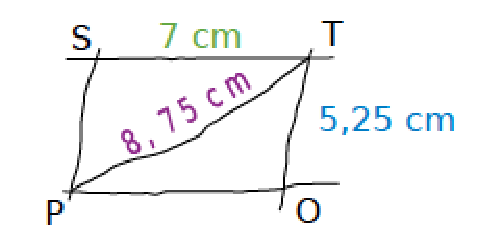
\includegraphics[scale=0.45]{GP1}
\end{center}
\end{minipage}
\end{exercice}


\begin{exercice}[]
Sur la figure ci-contre :

\begin{minipage}{0.6\linewidth}
\begin{itemize}
\item EFGH est un rectangle ;
\item EF = 14 m \emph{et} FG = 12 m ;
\item K $\in$ [EH] \emph{et} EK = 4 m ;
\item L $\in$ [EF] \emph{et} EL = 6 m.
\end{itemize}
Le triangle KGL est-il rectangle ?

\end{minipage}
\hfill
\begin{minipage}{0.35\linewidth}
\begin{center}

\begin{tikzpicture}[x=0.17cm,y=0.17cm]
\draw[fill=black,fill opacity=0] (0.7415589313755807,0.0) -- (0.7415589313755808,0.7415589313755807) -- (4.540738858441183E-17,0.7415589313755807) -- (0.0,-0.0) -- cycle; 
\draw[fill=black,fill opacity=0] (13.25844106862442,12.0) -- (13.25844106862442,11.25844106862442) -- (14.0,11.25844106862442) -- (14.0,12.0) -- cycle; 
\draw[fill=black,fill opacity=0] (4.540738858441183E-17,11.25844106862442) -- (0.7415589313755808,11.25844106862442) -- (0.7415589313755807,12.0) -- (0.0,12.0) -- cycle; 
\draw[fill=black,fill opacity=0] (14.0,0.7415589313755807) -- (13.25844106862442,0.7415589313755808) -- (13.25844106862442,9.081477716882366E-17) -- (14.0,0.0) -- cycle; 
\draw (0.0,-0.0)-- (0.0,12.0);
\draw (0.0,12.0)-- (14.0,12.0);
\draw (14.0,12.0)-- (14.0,0.0);
\draw (14.0,0.0)-- (0.0,-0.0);
\draw (0.0,8.0)-- (6.0,12.0);
\draw (6.0,12.0)-- (14.0,0.0);
\draw (14.0,0.0)-- (0.0,8.0);
\begin{tiny}
\draw [color=black] (0.0,-0.0)-- ++(-1.0pt,-1.0pt) -- ++(2.0pt,2.0pt) ++(-2.0pt,0) -- ++(2.0pt,-2.0pt);
\draw[color=black] (-0.7,-0.7) node {H};
\draw [color=black] (14.0,0.0)-- ++(-1.0pt,-1.0pt) -- ++(2.0pt,2.0pt) ++(-2.0pt,0) -- ++(2.0pt,-2.0pt);
\draw[color=black] (14.8,-0.7) node {G};
\draw [color=black] (0.0,12.0)-- ++(-1.0pt,-1.0pt) -- ++(2.0pt,2.0pt) ++(-2.0pt,0) -- ++(2.0pt,-2.0pt);
\draw[color=black] (-0.5,12.8) node {E};
\draw [color=black] (14.0,12.0)-- ++(-1.0pt,-1.0pt) -- ++(2.0pt,2.0pt) ++(-2.0pt,0) -- ++(2.0pt,-2.0pt);
\draw[color=black] (14.5,12.8) node {F};
\draw [color=black] (0.0,8.0)-- ++(-1.0pt,-1.0pt) -- ++(2.0pt,2.0pt) ++(-2.0pt,0) -- ++(2.0pt,-2.0pt);
\draw[color=black] (-1,8) node {K};
\draw [color=black] (6.0,12.0)-- ++(-1.0pt,-1.0pt) -- ++(2.0pt,2.0pt) ++(-2.0pt,0) -- ++(2.0pt,-2.0pt);
\draw[color=black] (6,13) node {L};
\end{tiny}
\end{tikzpicture}
\end{center}
\end{minipage}
\end{exercice}

\serie{Théorème de Thalès}

\begin{exercice}[]
On suppose que (AB)$\parallel$(CD).

On a AB = 72, CD = 96, SC = 84 et SD = 72.
 
Trouver SA et SB.
\begin{center}
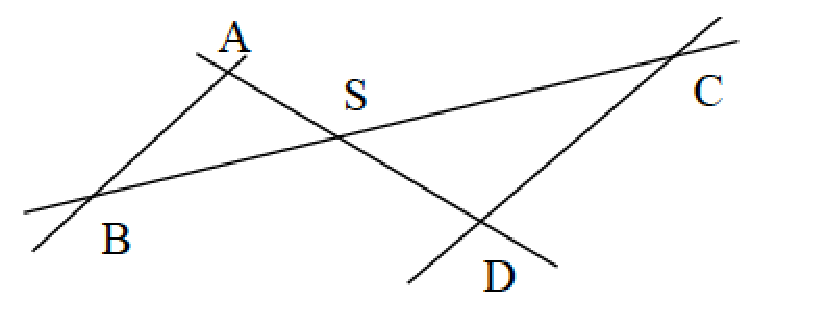
\includegraphics[scale=0.35]{GP2}
\end{center}
\end{exercice}

\begin{exercice}[]
On suppose que (AB)$\parallel$(CD) et que (AB)$\parallel$(EF).
 
AC= 10, CE = 15 et BD = 14.

Trouver DF.
\begin{center}
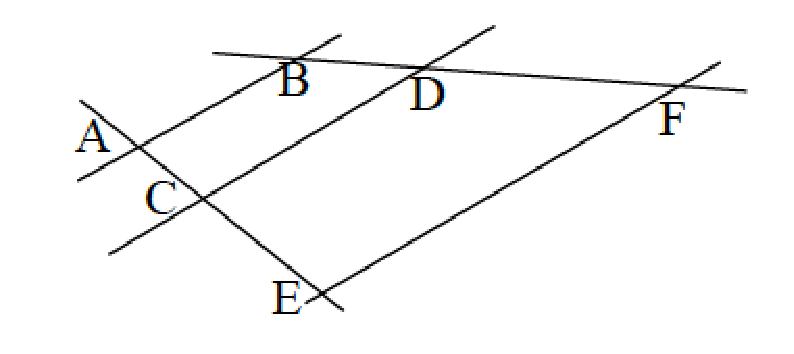
\includegraphics[scale=0.35]{GP3}
\end{center}
\end{exercice}

\begin{exercice}[]
On a : OM = 2,8 cm ; ON = 5,4 cm ; OS = 2,7 cm et OT = 1,4 cm.
Démontrer que les droites (MN) et (ST) sont parallèles.
\begin{center}
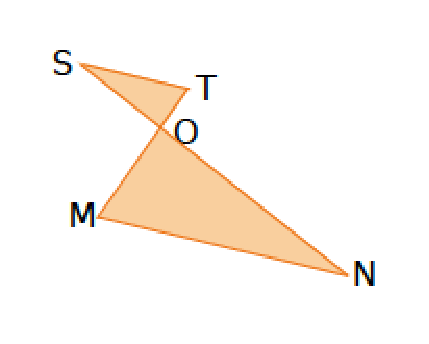
\includegraphics[scale=0.35]{GP4}
\end{center}
\end{exercice}

\begin{exercice}[]
L'unité de longueur choisie est le mètre. 
\begin{center}
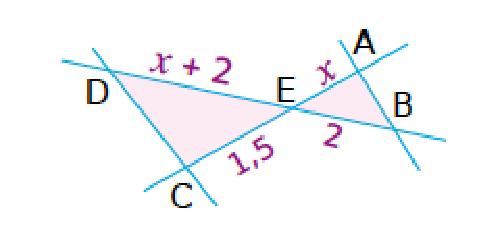
\includegraphics[scale=0.5]{GP7}
\end{center}

\begin{enumerate}
\item Pour $x = 2,5$, les droites (AB) et (CD) ne sont pas parallèles. 
Vrai ou faux? Expliquer la démarche.
\item Pour $x = 1$, les droites (AB) et (DC) ne sont pas parallèles. Vrai ou faux ? Expliquer la démarche.
\end{enumerate}
\end{exercice}

\begin{exercice}[]
Sur ce schéma les droites (EF) et (GH) sont sécantes en D.\\
Les droites (EG) et (FH) sont parallèles.\\
\begin{center}
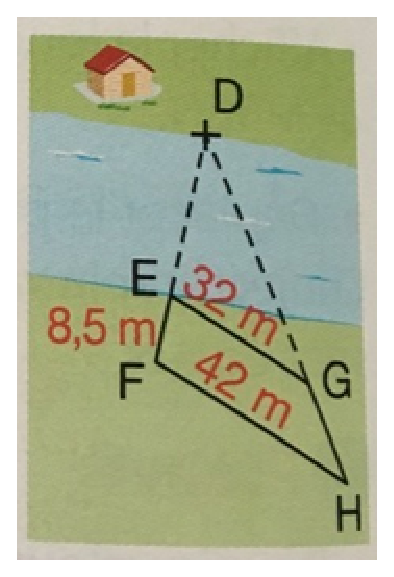
\includegraphics[scale=0.45]{GP10}
\end{center}
Quelle est la largeur DE de la rivière?
\end{exercice}

\serie{Divers}

\begin{exercice}[]
Sur la figure ci-dessous : GR=3,4 cm. 

Le point S est le milieu du côté [GR]. 

Calculer ST. 
\begin{center}
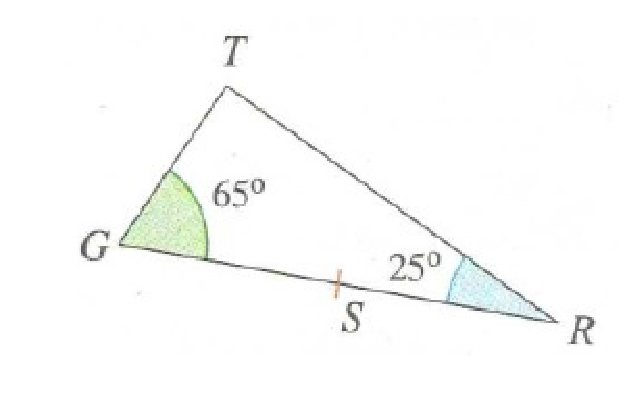
\includegraphics[scale=0.5]{GP5}
\end{center}
\end{exercice}

\begin{exercice}[]
Pour consolider un bâtiment, des charpentiers  ont construit un contrefort en bois (les mesures sont en mètre).

\begin{center}
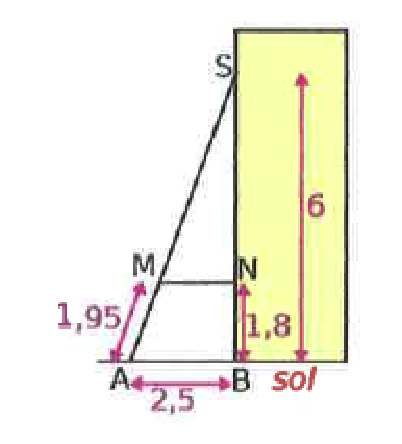
\includegraphics[scale=0.5]{GP8}
\end{center}

\begin{enumerate}
\item En considérant que le montant [BS] est perpendiculaire au sol, calculer la longueur AS.
\item Calculer les longueurs SM et SN.
\item Démontrer que la traverse [MN] est bien parallèle au sol.
\end{enumerate}
\end{exercice}

\begin{exercice}[]
Sur cette figure, C est un cercle de centre O et de rayon 3 cm.

La droite (d) est tangente en A au cercle C .

On voudrait calculer la longueur en cm du segment [OB].

1) Expliquer pourquoi on peut utiliser le théorème de Pythagore dans le triangle OAB.

2) Calculer l’arrondi au dixième de la longueur OB en cm.
\begin{center}
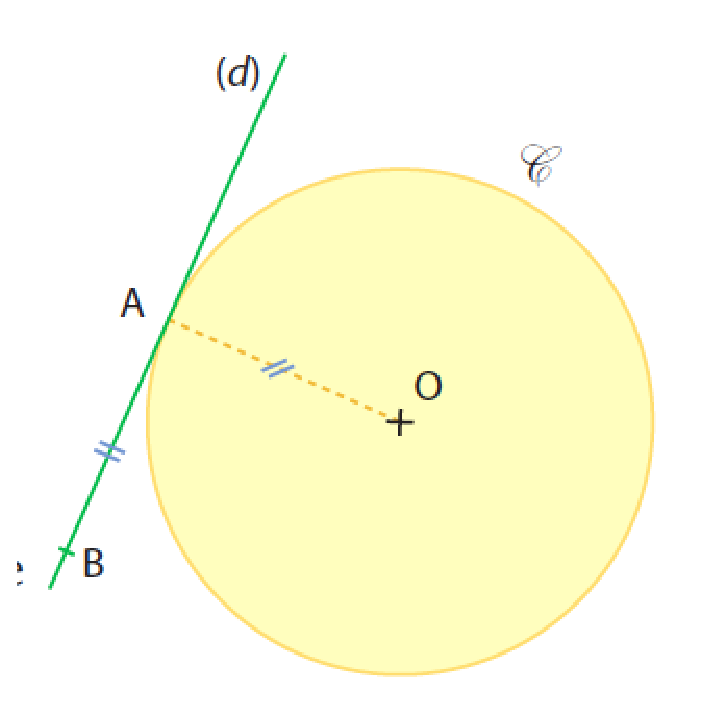
\includegraphics[scale=0.45]{GP6}
\end{center}
\end{exercice}

\begin{exercice}[]
Sur la figure, les droites (EF) et (MP) sont parallèles.
\begin{center}
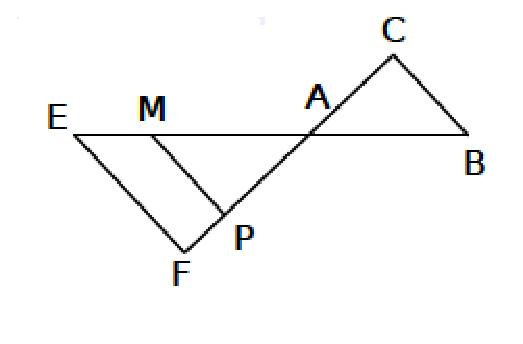
\includegraphics[scale=0.5]{GP9}
\end{center}

On sait que AM=6 cm ; MP=4,8cm ; AP=3,6 cm ; EF=6 cm ; AC=4,5 cm et AB=7,5 cm .

\begin{enumerate}
\item Démontrer que le triangle AMP est un triangle rectangle.
\item Calculer AE puis la longueur ME.
\item Démontrer que les droites (MP) et (BC) sont parallèles.
\end{enumerate}
\end{exercice}




\end{colonne*exercice}

\connaissances


\QCMautoevaluation{Pour chaque question, plusieurs réponses sont
  proposées.  Déterminer celles qui sont correctes.} % Est-ce que c'est toujours le cas ?

\begin{QCM}

\begin{GroupeQCM}

\begin{exercice}Si $RKE$ est rectangle en $K$ alors...
\begin{ChoixQCM}{4}
\item $RK^2 = RE^2 + EK^2$
\item $EK^2 = ER^2 + RK^2$
\item $RE^2 = RK^2 + KE^2$
\item $KE^2 = RE^2 – RK^2$
\end{ChoixQCM}
\begin{corrige}
\reponseQCM{b}
\end{corrige}
\end{exercice}

\begin{exercice}$ABC$ est rectangle en $A$ ; $AB = 5$ et $BC = 7$ (en cm). L'arrondi au dixième de $AC$ est...
\begin{ChoixQCM}{4}
\item 8,6 cm
\item 4,8 cm
\item 4,89 cm
\item 4,9 cm
\end{ChoixQCM}
\begin{corrige}
\reponseQCM{d}
\end{corrige}
\end{exercice}

\begin{exercice}Si $KG^2 \neq KC^2 + CG^2$ alors...
\begin{ChoixQCM}{4}
\item $KCG$ n'est pas rectangle
\item $KCG$ peut être rectangle
\item $KCG$ n'est pas rectangle en $C$
\item $KCG$ est quelconque
\end{ChoixQCM}
\begin{corrige}
\reponseQCM{b c}
\end{corrige}
\end{exercice}

\begin{exercice}

\definecolor{zzttqq}{rgb}{0.6,0.2,0.}
\begin{tikzpicture}[scale=0.75][line cap=round,line join=round,>=triangle 45,x=1.0cm,y=1.0cm]
\clip(1.16,0.4) rectangle (5.8,3.56);
\fill[color=zzttqq,fill=zzttqq,fill opacity=0.1] (2.,1.) -- (5.,1.) -- (5.,3.) -- cycle;
\draw [color=zzttqq] (2.,1.)-- (5.,1.);
\draw [color=zzttqq] (5.,1.)-- (5.,3.);
\draw [color=zzttqq] (5.,3.)-- (2.,1.);
\draw (4.,1.)-- (3.98461538462,2.32307692308);
\begin{scriptsize}
\draw [color=black] (2.,1.)-- ++(-1.5pt,-1.5pt) -- ++(3.0pt,3.0pt) ++(-3.0pt,0) -- ++(3.0pt,-3.0pt);
\draw[color=black] (1.66,1.14) node {$C$};
\draw [color=black] (5.,1.)-- ++(-1.5pt,-1.5pt) -- ++(3.0pt,3.0pt) ++(-3.0pt,0) -- ++(3.0pt,-3.0pt);
\draw[color=black] (5.26,1.02) node {$B$};
\draw [color=black] (5.,3.)-- ++(-1.5pt,-1.5pt) -- ++(3.0pt,3.0pt) ++(-3.0pt,0) -- ++(3.0pt,-3.0pt);
\draw[color=black] (5.14,3.28) node {$A$};
\draw [color=black] (4.,1.)-- ++(-1.5pt,-1.5pt) -- ++(3.0pt,3.0pt) ++(-3.0pt,0) -- ++(3.0pt,-3.0pt);
\draw[color=black] (4.,0.8) node {$N$};
\draw [color=black] (3.98461538462,2.32307692308)-- ++(-1.5pt,-1.5pt) -- ++(3.0pt,3.0pt) ++(-3.0pt,0) -- ++(3.0pt,-3.0pt);
\draw[color=black] (3.92,2.78) node {$M$};
\end{scriptsize}
\end{tikzpicture}

Si $M\in [AC]$, $N\in [BC]$ et $(MN)//(AB)$ alors...

\begin{ChoixQCM}{4}
\item $\dfrac{AM}{AC}=\dfrac{BN}{BC}=\dfrac{MN}{AB}$
\item $\dfrac{CM}{CN}=\dfrac{CA}{CB}=\dfrac{MN}{AB}$
\item $\dfrac{CM}{CA}=\dfrac{CN}{CB}=\dfrac{MN}{AB}$
\item $\dfrac{CM}{CA}=\dfrac{CB}{CN}=\dfrac{MN}{AB}$
\end{ChoixQCM}
\begin{corrige}
\reponseQCM{c}
\end{corrige}
\end{exercice}

\begin{exercice}Dans le cas précédent,  $CM = 4,5$ ; $MA = 3$ et $CN = 3$ donc...
\begin{ChoixQCM}{4}
\item $CB = 2$
\item $CB = 5$
\item $BN = 2$
\item $CB = \dfrac{9}{5}$
\end{ChoixQCM}
\begin{corrige}
\reponseQCM{b}
\end{corrige}
\end{exercice}


\begin{exercice}

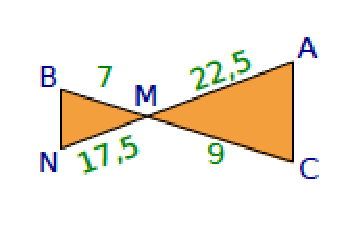
\includegraphics[scale=0.5]{GP11}
\begin{ChoixQCM}{4}
\item $(AC)$ et $(BN)$ sont parallèles
\item $(AC)$ et $(BN)$ ne sont pas parallèles
\item On ne peut pas savoir si $(AC)$ 
et $(BN)$ sont parallèles
\item $\dfrac{NB}{AC}=\dfrac{MB}{MC}$
\end{ChoixQCM}
\begin{corrige}
\reponseQCM{a d}
\end{corrige}
\end{exercice}


\end{GroupeQCM}
\end{QCM}


\pagebreak






\themaC
\chapter{Inéquations}

\exercicesbase
\begin{colonne*exercice}

\serie{Inégalités}

\begin{exercice}[]
Complétez le tableau suivant :

\begin{center}
\renewcommand{\arraystretch}{2}
\begin{tabular}{|>{\centering\arraybackslash}p{1.8cm}|>{\centering\arraybackslash}p{2.9cm}|>{\centering\arraybackslash}p{2.1cm}|}
\hline
\rowcolor[gray]{0.8}Intervalle & Représentation graphique & Inégalités\\\hline
$[-4;8]$&&\\\hline
&&$x<7$\\\hline
$]-\infty;3]$&&\\\hline
$]0;7]$&&\\\hline
&&$x\geq -1$\\\hline
&&$2>x\geq -4$\\\hline
\end{tabular}
\end{center}
\end{exercice}

\begin{exercice}[]
Sachant que $a$ est un nombre tel que $a<3$, compléter par une inégalité:
\setlength{\columnseprule}{0pt}
\begin{multicols}{2}[\raggedcolumns]
\begin{enumerate}
\item $a+3 ...$
\item $a-3 ...$
\item $3a ...$
\item $-3a ...$
\item $3a-\pi ...$
\item $-3a+3 ...$
\end{enumerate}
\end{multicols}
\end{exercice}

\begin{exercice}[]
Soient $x$ et $y$ deux nombres réels tels que\\
$-3,5<x<-3,4$ et $2,5<y<2,6$, encadrer les nombres suivants:
\setlength{\columnseprule}{0pt}
\begin{multicols}{2}[\raggedcolumns]
\begin{enumerate}
\item $4y+3$
\item $\dfrac{1}{4y+3}$
\item $7-3y$
\item $-xy$
\item $xy$
\end{enumerate}
\end{multicols}
\end{exercice}

\serie{Inéquations}
\begin{exercice}[]
Résoudre les inéquations suivantes :
\setlength{\columnseprule}{0pt}
\begin{multicols}{2}[\raggedcolumns]
\begin{enumerate}
\item $2x-4 \leq x-5$
\item ${2} + x \geq 3 x - 4$
\item ${2} x + {2} < {2} x - {4}$
\item $\dfrac{x -  {4}}{2} \leq  x - {1}$
\end{enumerate}
\end{multicols}
\end{exercice}

\begin{exercice}[]
Résoudre les inéquations suivantes :
\setlength{\columnseprule}{0pt}
\begin{multicols}{2}[\raggedcolumns]
\begin{enumerate}
\item ${2} (x - {1})  \geq  {2} x - {3}$
\item $x - \dfrac{1}{2} > {3} x - {4}$
\item $\dfrac{x} {5} + \dfrac{3}{10}   \leq {2}x$
\item $\dfrac{3 x - 14}{12} + \dfrac{3 x - 2}{4} > \dfrac{2 x - 1}{3}$
\end{enumerate}
\end{multicols}
\end{exercice}

\begin{exercice}[]
Résoudre les inéquations suivantes:
\setlength{\columnseprule}{0pt}
\begin{multicols}{2}[\raggedcolumns]
\begin{enumerate}
\item $3(x+1)-x\leq1+2(1+x)$
\item $-\dfrac{3}{5}x-6 < - \dfrac{2}{5}x+7$
\item $2x-\dfrac{2}{3}<2-\dfrac{x+1}{3}$ \\
\item $\dfrac{1}{5}-\dfrac{4}{3}\geq2\left( 1-\dfrac{5}{6}x\right) $
\end{enumerate}
\end{multicols}
\end{exercice}

\serie{Problèmes}
\begin{center}
\textit{Résoudre les problèmes suivants par une mise en inéquation.}
\end{center}
\begin{exercice}[]
Clément a 32 ans et Lucie a 5 ans.\\
Pendant combien d’années l’âge de Clément sera-t-il supérieur au quadruple de celui de Lucie ?
\end{exercice}

\begin{exercice}[]
Une session de karting coûte 55 CHF. Mais le prix passe à 11 CHF la session si vous 	achetez une carte d’abonnement à 900 CHF.\\
A partir de combien de session cet abonnement est-il avantageux ?
\end{exercice}

\begin{exercice}[]
Une famille espère économiser 250 CHF par an en récupérant de l’eau de pluie dans 	une citerne. Au bout de combien d’années les économies réalisées pourront-elles 	compenser l’achat de la citerne, qui coûte 910 CHF ?
\end{exercice}

\begin{exercice}[]
Maïa, nouvelle adhérente d’un club de squash, étudie les deux tarifs proposés :
\begin{description}
\item Tarif A : 55 CHF la séance;
\item Tarif B : achat d’une carte privilège annuelle de 400 CHF, donnant droit au tarif réduit de 40 CHF.
\end{description}
Pour combien de séances est-il plus avantageux d’acheter la carte privilège ?
\end{exercice}

\begin{exercice}[]
Un aller-retour en train entre deux villes coûte 80 CHF. Avec un abonnement annuel à 442 CHF, on bénéficie d’une réduction de $50\%$ sur le prix d’un aller-retour.\\
Quelle formule doit-on choisir en fonction du nombre de voyages effectués ?
\end{exercice}
	
\begin{exercice}[]
La somme de trois entiers consécutifs est comprise entre 367 et 372.\\ 
Quels sont ces entiers ?
\end{exercice}
	
\begin{exercice}[]
La largeur d’un terrain rectangulaire est égale à la moitié de sa longueur.\\
Ce terrain est entouré d’une allée de 1 m de large.\\
On sait que l’aire de l’allée est comprise entre 112 m$^{2}$ et 208 m$^{2}$.\\
Encadrez le plus précisément possible la largeur de ce terrain.\\\\\\\\\\\\
\end{exercice}

\begin{exercice}[]
Un bureau de recherche emploie 27 informaticiens et 15 mathématiciens. 

On envisage d’embaucher le même nombre $x$  d’informaticiens et de mathématiciens.

Combien faut-il embaucher de spécialistes de chaque sorte pour que le nombre de mathématiciens soit au moins égal aux deux tiers du nombre d’informaticiens ?\\
\end{exercice}

\begin{exercice}[]
La longueur d’un rectangle dépasse de 7 dm sa largeur. 

On sait que son périmètre est compris entre 20 dm et 26 dm. 

Que peut-on dire au sujet de sa largeur ?

\end{exercice}
\end{colonne*exercice}

\connaissances


\QCMautoevaluation{Pour chaque question, plusieurs réponses sont
  proposées.  Déterminer celles qui sont correctes.} 

\begin{QCM}
  \begin{GroupeQCM} 
  
    \begin{exercice}
      Parmi les nombres suivants, des solutions de l'inéquation
$2x + 7 \leq 3x + 5$ sont...
      \begin{ChoixQCM}{4}
      \item $-1$
      \item 0
      \item 3
      \item 2
      \end{ChoixQCM}
\begin{corrige}
     \reponseQCM{cd} 
   \end{corrige}
    \end{exercice}
    
    \begin{exercice}
      Le nombre 3 est solution de l'inéquation...
      \begin{ChoixQCM}{4}
      \item $3x+7<x-3$
      \item $2x-5\geq 1$
      \item $4x-4>x+1$
      \item $(x+7)^2>80$
      \end{ChoixQCM}
\begin{corrige}
     \reponseQCM{bcd} 
   \end{corrige}
    \end{exercice}
    
    \begin{exercice}
      L'inéquation qui a pour solutions tous les nombres  inférieurs ou égaux à $-2$  est...
      \begin{ChoixQCM}{4}
      \item $3x<-6$
      \item $x+2\geq 4x+8$
      \item $-5x\leq10$
      \item $8\geq x+10$
      \end{ChoixQCM}
\begin{corrige}
     \reponseQCM{bd} 
   \end{corrige}
    \end{exercice}
    
     \begin{exercice}
      $3x+2 \leq 2x + $1 possède exactement les mêmes solutions que...
      \begin{ChoixQCM}{4}
      \item $3x\leq 2x-1$
      \item $2x+1 \geq 3x+2$
      \item $x\leq 1$
      \item $-x \geq -1$
      \end{ChoixQCM}
\begin{corrige}
     \reponseQCM{ab} 
   \end{corrige}
    \end{exercice}
    
    \begin{exercice}
      Un nombre est supérieur ou égal à $-3$ donc...
      \begin{ChoixQCM}{4}
      \item son triple est strictement supérieur 
à $-3$
      \item son opposé est inférieur 
ou égal à 3
      \item son double peut être égal à $-10$
      \item en ajoutant 5, le résultat 
est positif
      \end{ChoixQCM}
\begin{corrige}
     \reponseQCM{bd} 
   \end{corrige}
    \end{exercice}
    
        \begin{exercice}
      L'inéquation $2x + 5 \leq 2x + 6$...
      \begin{ChoixQCM}{4}
      \item n'a pas 
de solution
      \item admet 7 comme solution
      \item a une infinité de solutions
      \item admet tout nombre positif comme solution
      \end{ChoixQCM}
\begin{corrige}
     \reponseQCM{bcd} 
   \end{corrige}
    \end{exercice}


\end{GroupeQCM}
\end{QCM}

  

\pagebreak







%\themaG
%\include{Quadrilateres/Quadrilateres}

%\themaC
%\include{NbsRelatifs/NbsRelatifs}

%\themaG
%\include{PerimetresAires/PerimetresAires}

%\AfficheListeMethodes
\AfficheCorriges[2]
%\AfficheLexique

\end{document}

%%% Local Variables: 
%%% mode: latex
%%% TeX-master: t
%%% End: 
